\documentclass[a4paper,10pt]{report}

% Packages
\usepackage{geometry}
\usepackage{makeidx}
\usepackage{srcltx}
\usepackage{multirow}
\usepackage{graphicx}
\usepackage{array}
\usepackage{wrapfig}
\usepackage{textcomp}

% Setup margins
\geometry{a4paper,left=2.5cm,right=2.5cm,top=2cm,bottom=2cm,includeheadfoot}

% Create index
\makeindex

\begin{document}

% New List Environment
\newenvironment{optlist}[1]
  {
    \begin{flushleft}\textbf{#1}\end{flushleft}
    \begin{list}{}{}
  }
  { \end{list} }

% User-Defined Commands
\newcommand{\progname}{{\sffamily Aten}}
\newcommand{\qte}[1]{\lq{}#1\rq{}}
\newcommand{\ttqte}[1]{\lq{}{\ttfamily#1}\rq{}}
\newcommand{\dqte}[1]{``#1''}
\newcommand{\its}{\hspace{20cm}}

\title{\progname{} version 0.91a \\ User's Guide}
\author{T. Youngs}
\maketitle

\tableofcontents

\clearpage

\section{Introduction}

\progname{} is first and foremost an application to ease the creation of coordinates suitable for use as the starting configurations for molecular simulation codes, ranging from single molecules \textit{in vacuo} to condensed-phase systems such as gases or liquids. Forcefield methods can be applied, for example, to minimise the energy of systems with respect to their coordinates and create \qte{good guesses} for initial configurations as input to \textit{ab initio} codes. More so, multi-molecule models can be created with Monte Carlo techniques to provide periodic systems for use in molecular dynamics.\\

For the computional chemist, it is often the case that coordinates (new or existing) need to be edited in a specific way to create the configuration necessary to perform the job at hand, and in the opinion of the author, this is a job not handled well by current the current stock of free codes available. \progname{} was initially created as a method of learning various programming, visual, and algorithmic techniques, but has grown into an application suitable for use in many situations by the simulation community.\\

Comments and suggestions on the facilities available (or not) in the code are welcome and will be warmly accepted. If a feature is missing or inadequate and of general applicability, I will most likely include it in the program. Please don't hesitate to write to me at the address provided below. In particular, if you take the time to write a file filter for use with your favourite code I would be happy to include as part of the distribution.\\

\progname{} is released under the GPL, meaning you may copy, change, and distribute it as you see fit, provided you acknowledge the original copyright. If, however, you have a burning desire to improve or extend the code in some way, and wish to do some under your own steam, I would be happy to consider including your modifications into the official stream. Contact me to discuss your brilliance at interpreting my code!\\

Tristan Youngs\\
9$^\textrm{th}$ November 2007\\
t.youngs@qub.ac.uk\\

% Include sections
\chapter{Installation}
\label{sec:install}

\section{\emph{Disclaimer}}
\label{sec:disclaimer}

\progname{} has been compiled successfully on Linux machines running SuSE 9.3 (with the GTK gui), OpenSuSE 10.2, and RedHat Enterprise 4, an Intel iMac running OS X 10.4.10, and XXX. No doubt with (or without) tweaking it will run on other systems.\\

\progname{} is in development, and as such might contain a bug or two. Should you come across a crash or an issue that needs to be fixed, \emph{please} report them so they can be fixed.\\

In addition, I can't accept responsibility for any loss of data / work / sleep / expensive computers / cats / coordinates etc., use at your own risk etc., and so on...\\

\section{Ingredients for Linux}
\label{sec:linuxinstall}
\begin{itemize}
	\item GNU Autotools 2.6
	\item A C++ compiler (e.g. g++, icc)
	\item OpenGL and glut (e.g. from freeglut)
	\item pkg-config
	\item GTK+2.0 (version 2.4 or above) or Qt4 (version 4.2 or above) if you want a GUI
	\item GtkGLExt if you want the GTK+ GUI
\end{itemize}

\section{Ingredients for Mac OS X}
\label{sec:macinstall}
\begin{itemize}
	\item GNU Autotools 2.6
	\item A C++ compiler (e.g. g++, icc)
	\item OpenGL and glut frameworks
	\item pkg-config (if using Fink or MacPorts versions of GTK+ or Qt)
	\item GTK+ (version 2.4 or above) or Qt (version 4.1 or above) if you want a GUI
\end{itemize}

\subsection{Which Qt4?}

To build against the qt4-x11 package available $via$ Fink run:\\

\indent {\sffamily configure {-}{-}with-qt=fink} ...\\

This will set most of the necessary environment variables, namely:\\
{\sffamily
\begin{itemize}
	\item QTGUI\_CFLAGS='-I/sw/lib/qt4-x11/include -I/usr/X11R6/include'
	\item QTGUI\_LIBS='-L/sw/lib/qt4-x11/lib -lQtGui -lQtCore -lQtOpenGL'
	\item QTOPENGL\_CFLAGS='-I/sw/lib/qt4-x11/include'
	\item QTOPENGL\_LIBS='-I/sw/lib/qt4-x11/lib'
\end{itemize}
}

You may also need to direct the build process to the correct Qt4 development binaries either by setting your \$PATH to \qte{/sw/lib/qt4-x11/bin:\$\{PATH\}} or by using the {\sffamily {-}{-}with-qtdir} option to {\sffamily configure}.\\

The native Qt4 package is available as a disk image installer at no cost directly from http://trolltech.com. Specify that the build use the frameworks provided instead:\\

\indent {\sffamily configure {-}{-}with-qt=framework} ...\\

\subsection{Autotools}
You may find that the version of GNU Autotools you have is not recent enough. Check with {\sffamily autoconf {-}{-}version} - 2.59 is not sufficient! An up-to-date version can be installed via Fink. Known good versions are listed here, but don't assume that these are the only versions that will work:\\

{\sffamily
\indent libtool  :  1.5.22-1000\\
\indent autoconf :  XXX\\
\indent automake :  1.9.6-3\\
}

\section{Configuration Options}

Possible {\sffamily configure} options are listed here. Most are present just to work around compilation issues, but some provide functionality in the program (in particular, the choice of GUI to build in).

\begin{description}

	\item[{-}{-}with-gl-includedir]
		Sets the location of the OpenGL headers.
	\begin{description}
		\item[e.g. {-}{-}with-gl-includedir=/usr/include]
			Sets the location of the OpenGL headers (GL/GL.h etc.) to /usr/include.
	\end{description}

	\item[{-}{-}with-gui] Specifies GUI to compile with the program. Valid options are:
	\begin{description}
		\item[{-}{-}with-gui=none\its]
			No GUI should be compiled (i.e. create a command-line only version)
		\item[{-}{-}with-gui=gtk\its]
			Compile the legacy GTK+ GUI.
		\item[{-}{-}with-gui=qt\its]
			Compile the Qt4 GUI (default).
	\end{description}

	\item[{-}{-}with-qt] Specifies which installation of Qt4 to use on Apple Macs. Valid options are:
	\begin{description}
		\item[{-}{-}with-qt=framework]
			Use the Qt4 framework provided by TrollTech's own installation.
		\item[{-}{-}with-qt=fink]
			Use the Fink installation of Qt4 (qt4-x11).
	\end{description}

	\item[{-}{-}with-qtdir] Sets the location of the Qt4 development tools ({\sffamily moc}, {\sffamily uic}, and {\sffamily rcc}). This should only need to be set if you have Qt3 installed and your \$PATH favours the older version's binaries.
	\begin{description}
		\item[e.g. {-}{-}with-qtdir=/usr/local/bin]
			Sets the location of the Qt4 development tools to /usr/local/bin.
	\end{description}

\end{description}


\section{Four Step Installation}

\begin{description}
	\item[Step 1:\its] Get the source.
	\begin{itemize}
		\item Download the source distribution from the website and unpack the .tgz file, or get the latest tree from the SVN repository.
		\item Run {\sffamily ./autogen.sh} to generate the {\sffamily configure} script if you got the distribution using svn.
	\end{itemize}
	Common issues:\\
	\emph{(MAC) Running {\sffamily ./autogen.sh}, autoconf fails with \qte{configure.ac:16: error: possibly undefined macro: AC\_DEFINE}.}
	\begin{itemize}
		\item This is related to the version of pkg-config you have installed (e.g. version 0.15.1 gives this error, but version 0.21 does not) with Fink / MacPorts. Upgrade to the latest version. Incidentally, the line-number reported (16) is not the actual location of the error -- autoconf reports this wrongly (the actual error occurs around line 89 with the \qte{PKG\_CHECK\_MODULES(GTK28, ..., [AC\_DEFINE...} command).
	\end{itemize}
\end{description}

\begin{description}
	\item[Step 2:\its] Configure the build (Run {\sffamily./configure})
	\begin{itemize}
		\item Most all dependencies should be detected by the scripts provided, ensuring a pain-free build (or quick detection of problems).
		\item Select a GUI. Running {\sffamily./configure} with no options detects the operating system and builds in the Qt GUI. This can be overriden with the {\sffamily {-}{-}with-gui} switch:
		\begin{itemize}
			\item {\sffamily./configure {-}{-}with-gui=qt} builds in the Qt GUI (default).
			\item {\sffamily./configure {-}{-}with-gui=gtk} builds in the legacy GTK+ GUI.
			\item {\sffamily./configure {-}{-}with-gui=none} builds a command-line only executable.
		\end{itemize}
	\end{itemize}
	Common issues:\\
	\emph{$configure$ complains \dqte{Could not find GLUT header. Is freeglut/Mesa installed?}}
	\begin{itemize}
		\item You need some form of OpenGL implementation installed. Try the freeglut packages, and don't forget to install the freeglut-devel package as well.
	\end{itemize}
\end{description}

\begin{description}
	\item[Step 3:\its] Compile the source (Run {\sffamily make})
	\begin{itemize}
		\item Once configured successfully, run {\sffamily make} to compile the source and build the program.
		\item Go make some tea or brew some coffee.
	\end{itemize}
	Common issues:\\
	\emph{When linking I get \dqte{Undefined references to \qte{pango\_x\_font\_subfont\_xlfd}} (or similar).}
	\begin{itemize}
		\item The version of gtkglext you have installed is a bit retro (version 1.0.6 uses tokens from the pango subsystem that have since been made obsolete) so download and install version 1.2.0 from gtkglext.sourceforge.net.
	\end{itemize}
	\emph{When the Qt GUI is building, I get a version error for {\sffamily moc} along the lines of \qte{uic: File generated with too recent version of Qt Designer (4.0 vs. 3.*.*)}.}
	\begin{itemize}
		\item If you have both Qt4 and Qt3 installed \$PATH is often set so that the Qt3 binaries are found first. Reconfigure the build with {\sffamily configure {-}{-}with-qdtir=$path$} where $path$ is the location of the Qt4 binaries {\sffamily moc}, {\sffamily uic}, and {\sffamily rcc}.
	\end{itemize}

\end{description}

\begin{description}
	\item[Step 4:\its] Install (Run {\sffamily make install} or {\sffamily cp src/aten $<$destination$>$})
	\begin{itemize}
		\item After compilation is complete, you're left with the \progname{} executable in the src/ directory.
		\item Either run {\sffamily make install} to place the program in {\sffamily /usr/local/bin} if you have root priveledges, or copy the program to a local location of your choice and run it from there.
		\item The default stock of filters and spacegroup definitions is installed in the default locations if you run {\sffamily make install} (on Linux systems this is typically /usr/local/share/aten).
		\item Aten is directed to this location via the \$ATENDATA environment variable which should be set before running the program.
		\item If you haven't (or can't) run {\sffamily make install} then set \$ATENDATA to the /data directory in the source tree.
	\end{itemize}
\end{description}



\chapter{Quickstart}
\label{sec:quickstart}
Each user using \progname{} needs a $.aten$ directory in their home directory. Within this directory live files needed by the program, such as the user's own preferences, element colour scheme, etc. Some of these the program can do without -- others will result in errors on startup. Included in the archive is an archive named \qte{dotaten.tgz} which contains standard copies of the preferences file, spacegroup list, and file filters, and should be unpacked in the home directory (see Section \ref{sec:install}).\\


\section{Startup}
\label{sec:startup}
Several files are processed before the main program begins, in a set order:\\

\begin{description}
\item[{\it \qte{\$HOME/.aten/spgrp.dat}}\its]
	{\it XXX Should be installed rather than read from user directory}. Symmetry operations for the 230 spacegroups are read from here. If the file cannot be found the program will start as normal, but crystal packing will not be available.

\item[{\it \qte{\$HOME/.aten/filters/index}}\its]
	{\it XXX Read from installed location as well as user directory?}. A list of import/output filters to be found in the this directory are given in the \qte{index} file, one per line. If the file cannot be found, no filters are read and consequently no import or export will be possible, and so the program exits.

\item[{\it \qte{\$HOME/.aten/prefs.dat}}\its]
	User preferences controlling program behaviour, input methods, colours etc. are read last. If the file cannot be found, defaults are used and the program starts as normal. For a full list of possible options see Section \ref{sec:prefs}.

\end{description}

Run from the command line without arguments, \progname{} starts up with the full GUI. If model files are given as arguments, these are loaded after the above actions have completed. Whether a model file is readable and/or writable by \progname{} is determined by the current stock of filters available to the program (read from \qte{\$HOME/.aten/filters} and XXX). Many command-line options exist to allow for immediate loading of models, scripts, forcefields etc., and run the program in batch mode. See Section \ref{sec:cli} for a full list.\\


\section{Main Window}
Most of the main window is taken up with a canvas which is used to display and edit models and take input from the user. Each of the mouse buttons has a different action on the canvas, each of which can be set to the users taste in the preferences (see Section \ref{sec:preferences}). In addition the Shift, Ctrl, and Alt keys modify or augment these default actions. See the following sections for brief descriptions of the different modes. At the foot of the window is a message box (where output and errors are thrown) and a status bar reflecting the content of the current model displayed, listing the number of atoms and the number of selected atoms (bold value in parentheses, but only if there are selected atoms), the mass of the model, and the cell type and density of the model (if it is periodic).

{\it XXX Trajectory Frame number???}

A toolbar on the left-hand side of the window provides quick access to common functions. The first four manage models and the visible items in the main window. From the top down these are: toggle model list, add new model, delete current model, and toggle message box. The model list (hidden by default) appears on the right-hand side of the window and gives access to all the models currently loaded. Adding a new model will also add it to this list. The visibility of both the model list and the message box can be toggled with the relevant buttons giving more space to the main canvas.

\section{Changing the View}
At its most basic the canvas acts as a visualiser allowing the model to be rotated, zoomed in and out, and drawn in various different styles. By default, the right mouse button is used to rotate the molecule in the plane of the screen (right-click and hold on an empty area of the canvas and move the mouse to rotate the model) and the mouse wheel zooms in and out. Note that right-clicking on an atom brings up the atom menu (see Section \ref{sec:atommenu}). The middle mouse button translates the model in the plane of the screen -- again, click-hold and drag. Rotation and translation operate on the position and orientation of the camera and no modifications to the actual coordinates of the model are made. The view can be reset at any time from the main menu (View$\rightarrow$Reset) or by pressing Ctrl-R. Both the main menu (View$\rightarrow$Model Style) and the left-hand toolbar allow the drawing style of the model to be changed between stick, tube, sphere, scaled sphere, and \qte{individual}. The last option allows different view styles to be set for different atoms.\\

The Ctrl key changes the normal behaviour of the rotation and translation operations and forces them to be performed on the coordinates of the current atom selection instead of the camera. The centre of rotation is the geometric centre of the selected atoms.

\section{Selection}
Atom selection or picking is performed with the left mouse button -- hovering the mouse over an atom will emphasise it by drawing a circle around the edge of the atom, indicating that it can be single-clicked to highlight (select) it. Single-clicks perform \qte{exclusive} selections; that is, all other atom(s) are deselected before the clicked atom is (re)selected. Double-clicking on an atom brings up the atom list (see Section XXX). Clicking in an empty region of the canvas deselects all atoms. Clicking on an empty space in the canvas, holding, and dragging draws a rectangular selection region -- releasing the mouse button then selects all atoms whose screen coordinates are within this area. Again, this selection operation is exclusive. Inclusive selections (where already-selected atoms are not deselected) is performed by holding the Shift key. Furthermore, single-clicking on a selected atom while holding Shift will deselect the atom.\\


Out of the box the standard settings are:\\

\begin{table}[h!]
  \caption{}
  \begin{tabular}{cc|l}
\hline
	Button	& Modifier	& Action \\
\hline
	Left	& None		& Click on individual atoms to select exclusively \\
		&		& Click-hold-drag to exclusively select all atoms within rectangular region \\
		&		& Double-click to show atom list \\
		& Shift		& Click on individual atoms to toggle selection state \\
		&		& Click-hold-drag to inclusively select all atoms within rectangular region \\
\hline
	Right	& None		& Click-hold-drag to rotate camera around model \\
		&		& Click on atom to show atom menu \\
		& Ctrl		& Click-hold-drag to rotate selection in local (model) space \\
\hline
	Middle	& None		& Click-hold-drag to translate camera \\
		& Ctrl		& Click-hold-drag to translate selection in local (model) space \\
  \end{tabular}
\end{table}


\section{Load it!}
\label{sec:loadit}
If the names of model files are supplied on the command line, all are loaded into the workspace, their file formats determined by file extensions and/or content and parsed accordingly. Should the name of only one model be provided, the model list in the main view will be hidden. If none of the supplied files can be loaded, the program will exit without starting the GUI. The GUI can be suppressed for when batch command-line operation is required.\\

\progname{} uses \qte{filters} to achieve import and export of model file types, potentially providing the ability to load and save any format of model data available. A filter consists of a series of commands describing the layout of the data in a given file type, and may be thought of as a small, simplified C program typically of a few tens of lines in size. Thus, filters may be written by the user to enable the import/export of data in formats tailored to the need of the individual, or to read proprietary formats not in common usage within the community. See section \ref{sec:filterhandbook} for full details on using and writing filters. \\


%\subsection{General Considerations}
%\label{sec:genfiles}

%All input files (the preferences file, forcefields, scripts etc.) for \progname{} are entirely free-format. Comments, lines beginning with a hash (\qte{\#}), are always ignored, as are blank lines (or lines containing only delimiters) in the majority of cases. Valid delimiters between datum are spaces, commas, and tabs, although all these may be overruled by the use of double or single quotes to specify, for example, filenames or titles that contain any of the delimiters. For model loading, any or all of these rules may not apply since specific formatting may bypass any or all of these rules.





\chapter{Features}

\progname{} was designed with the needs of the molecular dynamics user in mind, but is more than likely to be useful in more general situations as well. At its simplest, it is (another) visualiser -- at its most complex, it is a forcefield-based tool for the creation and editing of gas- and liquid-phase configurations, offering an advanced atom typing system, energy minimisation, Monte Carlo methods for the creation of disordered systems, energy / force calculation, and tools for analysis.\\

\begin{optlist}{In a nutshell:}
	\item Load, display, save (images or coordinates) model files.
	\item Draw, edit, add, delete, move, position, and rotate atoms.
	\item Display, add, and edit unit cells (including spacegroup packing).
	\item Load and apply atom typing and forcefield terms to models.
	\item Calculate energies / forces.
	\item Geometry minimise structures.
\end{optlist}

Detailed feature information:\\

\begin{optlist}{Visualising}
	\item Visualise molecules / systems / trajectories in glorious line, tube, sphere and scaled sphere styles (or an arbitrary mix).
	\item Play movies of molecular dynamics trajectories.
	\item Save image snapshots.
\end{optlist}

XXX More!

\chapter{Using as a GUI Application}
\label{sec:gui}
\index{gui}

\section{The Main Window}
\index{gui!main window}

Most of the main window is taken up with a canvas which is used to display and edit models and take input from the user. A set of tabs directly above the main view shows the title of each loaded model currently available. The model being displayed on the main canvas (the \qte{current} model) is the one for which all input and editing tools will act on. \\

Each of the mouse buttons has a different action on the canvas, each of which can be set to the users taste in the preferences (menu item Settings$\rightarrow$Preferences on Linux). In addition the Shift, Ctrl, and Alt keys modify or augment these default actions. See the following sections for brief descriptions of the different modes. At the foot of the window is a message box (where output and errors are thrown) and a status bar reflecting the content of the current model displayed, listing the number of atoms and the number of selected atoms (bold value in parentheses, but only if there are selected atoms), the mass of the model, and the cell type and density of the model (if it is periodic).\\

A stack of icons on the right-hand side of the window provides quick access to different tool panels for building, analysing etc. The icons are:\\

\noindent
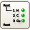
\includegraphics[width=1cm]{images/stack_atomlist} Shows a list of atoms in the model \\

\includegraphics[width=1cm]{images/stack_cell} Add, edit, or transform the model's unit cell \\

\includegraphics[width=1cm]{images/stack_edit} Tools to edit atoms and bonds \\

\includegraphics[width=1cm]{images/stack_transform} Transform selections of atoms \\
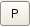
\includegraphics[width=1cm]{images/stack_position} Position selections of atoms \\

\includegraphics[width=1cm]{images/stack_ff} Load and edit forcefields, and assign to models and patterns \\
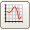
\includegraphics[width=1cm]{images/stack_minimise} Minimise the energy of models \\

\includegraphics[width=1cm]{images/stack_disorder} Create disordered systems \\

See the relevant sections of the manual for descriptions of each of these panels.

\section{Changing the View}
\index{gui!visualisation}

At its most basic the canvas acts as a visualiser allowing models to be rotated, zoomed in and out, and drawn in various different styles. By default, the right mouse button is used to rotate the molecule in the plane of the screen (right-click and hold on an empty area of the canvas and move the mouse to rotate the model) and the mouse wheel zooms in and out. Note that right-clicking on an atom brings up the atom menu (see Section \ref{sec:atommenu}). The middle mouse button translates the model in the plane of the screen -- again, click-hold and drag. Rotation and translation operate on the position and orientation of the camera and no modifications to the actual coordinates of the model are made. The view can be reset at any time from the main menu (View$\rightarrow$Reset) or by pressing Ctrl-R. Both the main menu (View$\rightarrow$Style) and the View toolbar allow the drawing style of models to be changed between stick, tube, sphere, scaled sphere, and individual. The last option allows different view styles to be set for different atoms.\\

The Ctrl key changes the normal behaviour of the rotation and translation operations and forces them to be performed on the coordinates of the current atom selection instead of the camera. The centre of rotation is the geometric centre of the selected atoms.

\section{Selection}
\index{gui!selections}

Atom selection or picking is performed with the left mouse button by default -- single-click on any atom to highlight (select) it. Single-clicks perform \qte{exclusive} selections; that is, all other atom(s) are deselected before the clicked atom is (re)selected. Clicking in an empty region of the canvas deselects all atoms. Clicking on an empty space in the canvas, holding, and dragging draws a rectangular selection region -- releasing the mouse button then selects all atoms within this area. Again, this selection operation is exclusive. Inclusive selections (where already-selected atoms are not deselected) are performed by holding the Shift key whil performing the above operations. Furthermore, single-clicking on a selected atom while holding Shift will deselect the atom.\\


To summarise mouse control, standard settings out of the box are:\\
\index{gui!mouse control}

\begin{table}[h!]
  \caption{}
  \begin{tabular}{cc|l}
\hline
	Button	& Modifier	& Action \\
\hline
	Left	& None		& Click on individual atoms to select exclusively \\
		&		& Click-hold-drag to exclusively select all atoms within rectangular region \\
		&		& Double-click to show atom list \\
		& Shift		& Click on individual atoms to toggle selection state \\
		&		& Click-hold-drag to inclusively select all atoms within rectangular region \\
\hline
	Right	& None		& Click-hold-drag to rotate camera around model \\
		&		& Click on atom to show atom menu \\
		& Ctrl		& Click-hold-drag to rotate selection in local (model) space \\
\hline
	Middle	& None		& Click-hold-drag to translate camera \\
		& Ctrl		& Click-hold-drag to translate selection in local (model) space \\
  \end{tabular}
\end{table}

\section{Main Menu}
\index{gui!main menu}

The following section lists the menu commands in Aten and the functions they perform, pointing to relevant sections in the remainder of the manual.

\subsection{File Menu}

\begin{table}[h!]
	\caption{}
	\begin{tabular}{cc|l}
		Item		& Shortcut	& Action \\
		\hline
		New Model	& Ctrl-N & Create a new, empty model, appearing in a new tab above the main view \\
		Load model	& Ctrl-L & Load an old model from disk, creating a new tab above the main view \\
		Recent Files	&	 & Lists the five most recently opened / edited files for quick access \\
		Add Trajectory	& 	 & Associate a trajectory on disk to the current model \\
		Save Model	& 	 & Save changes to the current model to its existing file or, if the model is newly-created, prompt for a filename to save to \\
		Save Model As	&	 & Prompt for a new filename to save the current model to \\

	\end{tabular}
\end{table}

% See Section \sec{}

\section{Toolbars}
\index{gui!toolbars}
\chapter{Forcefield Expressions}

A collection of atoms can live quite happily on its own in \progname{}, and can be moved around, rotated, deleted and added to at will. However, if you want to calculate the energy or forces of a collection of atoms (or employ methods that use such quantities) then a description of the interactions between the atoms is required. Creating a suitable $expression$ is the process of taking a system of atoms and generating a prescription for calculating the energy and/or forces arising from these interactions from any standard classical forcefield available.\\

On the way to generating an expression, several preliminary steps are performed:

\begin{enumerate}
	\item Detect molecule patterns for efficient usage of forcefield terms
	\item Augment bonds within (otherwise chemically \qte{correct}) molecules
	\item Find rings and assign aromaticity
	\item Assign atom hybridisation
\end{enumerate}

The first serves to enable the creation of optimal forcefield expressions for systems containing many copies of the same molecules (e.g. liquids), while the last three provide additional data beyond basic topology parameters for use in atom typing. All are performed automatically unless you specifically request them not to be (see Section XXX). The most important of these is the pattern description of the system, without which the expression cannot be created.

\section{Patterns}

Patterns describe systems in terms of their constituent molecular units. For an $N$-component system (a single, isolated molecule is a 1-component system) there are $N$ unique molecule types which are represented as, ideally, a set of $N$ patterns. Forcefield subexpressions can then be created for each pattern and applied to each molecule within it, allowing the expression for the entire system to be compact and efficient. Each pattern contains a list of intramolecular terms (bonds, angles etc.), atom types, and van der Waals parameters for a single molecule that can then be used to calculate the energy and forces of $M$ copies of the molecule.


From the atoms and the basic connectivity between them \progname{} will automatically determine the pattern of systems of arbitrary complexity. The ordering of atoms is important, however, and the atoms belonging to a single molecule must not be interspersed by those from others. In other words, if a bond \qte{crosses an atom} that doesn't belong to the molecule, then the benefits of fine-graining the expression in this way is lost somewhat. There are also many ways to represent the same system of atoms, all of which (from the point of view of the program) are equivalent and will produce the same total energies and atomic forces. Consider the following examples:

\begin{table}
\centering
\begin{tabular}{c c l}
	1. & \multirow{2}{*}{ 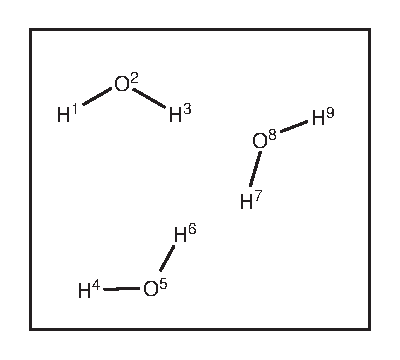
\includegraphics[width=3cm]{images/pattern1} } &
		Atom Order: H$^1$ O$^2$ H$^3$ H$^4$ O$^5$ H$^6$ H$^7$ O$^8$ H$^9$ \\
		& & Pattern: H$_2$O$(3)$ \\\\\\\\\\\\
	2. & \multirow{2}{*}{ 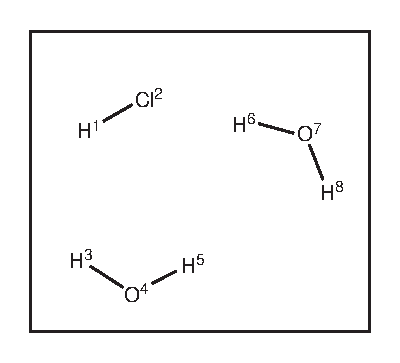
\includegraphics[width=3cm]{images/pattern2} } &
		Atom Order: H$^1$ Cl$^2$ H$^3$ O$^4$ H$^5$ H$^6$ O$^7$ H$^8$ \\
		& & Pattern: HCl$(1)$ H$_2$O$(2)$ \\\\\\\\\\\\
	3. & \multirow{2}{*}{ 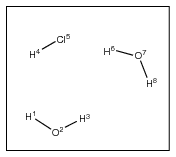
\includegraphics[width=3cm]{images/pattern3} } &
		Atom Order: H$^1$ O$^2$ H$^3$ H$^4$ Cl$^5$ H$^6$ O$^7$ H$^8$ \\
		& & Pattern: H$_2$O$(1)$ HCl$(1)$ H$_2$O$(1)$ \\\\\\\\\\\\
	4. & \multirow{2}{*}{ 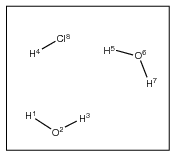
\includegraphics[width=3cm]{images/pattern4} } &
		Atom Order: H$^1$ O$^2$ H$^3$ H$^4$ H$^5$ O$^6$ H$^7$ Cl$^8$ \\
		& & Pattern: H$_5$O$_2$Cl$(1)$ \\\\\\\\\\\\
\end{tabular}
\end{table}


In 1) the three water molecules are identical with respect to the ordering of the atoms, so our description consists of a single pattern describing one H$_2$O. Obvious, huh? The two-component system illustrated in 2) and 3) is described by two different patterns since, in 3), the two water molecules are \qte{separated} by the hydrogen chloride. Thus, we end up with a three-pattern description to describe the contents of the system as opposed to the optimal two-pattern description, but remember that both are acceptable and will give the same total energies and atomic forces -- only the partitioning of the molecules has changed, and their order is not important (the actual positions of the atoms of course remains constant). This illustrates the point that molecules of the same type need not exist next to each other in terms of the overall atom list, but that the optimal pattern description will not be possible. There are likely to be many possible pattern descriptions for systems, some of which may be useful to employ, and some of which may not be. Take the well-ordered system 1) -- there are four ways to describe the three separate molecules:

\begin{enumerate}
	\item H$_2$O$(3)$
	\item H$_2$O$(1)$ H$_2$O$(1)$ H$_2$O$(1)$
	\item H$_2$O$(2)$ H$_2$O$(1)$
	\item H$_2$O$(1)$ H$_2$O$(2)$
\end{enumerate}

Again, all are equivalent and will give the same energies / forces. Sometimes it is useful to treat individual molecules as separate patterns in their own right since it allows for calculation of interaction energies with the rest of the molecules of the system. \\

Recall that bonds \qte{crossing atoms} will prevent the optimal description of atoms, but now consider that patterns can \qte{cross molecules}. For instance, consider again the example 1) above. Three further (again, reiterating the point, equivalent) ways of writing the pattern description are:

\begin{enumerate}
	\item H$_6$O$_3(1)$
	\item H$_4$O$_2(1)$ H$_2$O$(1)$
	\item H$_2$O$(1)$ H$_4$O$_2(1)$
\end{enumerate}

Here, we have encompassed individual molecular entities into supermolecular groups, and as long as there are no bonds \qte{poking out} of the pattern element, this is perfectly acceptable. Although this coarse-graining is a rather counter-intuitive way of forming patterns, it nevertheless allows them to be created for awkward systems such as that in 4) above. We may write two valid patterns for this arrangement of atoms:

\begin{enumerate}
	\item H$_5$O$_2$Cl$(1)$
	\item H$_2$O$(1)$ H$_3$OCl$(1)$
\end{enumerate}

Note that, when automatically creating patterns, if \progname{} stumbles across a situation like this, it will assume the default pattern of one supermolecule (the whole system of atoms), i.e. X$(1)$ where \qte{X} is all atoms. This will work, but will result in rather inefficient calculations.

\section{Creating the Expression}

For each element in the pattern the required intramolecular terms and atom types are determined for the representative molecule of the element. Atom typing is a complex process and is discussed in detail in Section \ref{sec:typing}. For now, let us assume that each atom in the molecules of each pattern element has been successfully assigned a forcefield type (if this cannot be achieved, then the expression cannot be created). Once \progname{} has convinced itself that every atom has type, a skeleton list of intramolecular terms (currently only bonds, angles, and torsions are supported) necessary to describe the element molecules is constructed and subsequently filled (\qte{fleshed out}) with parameters. These parameters come either from the forcefield associated to the model as a whole, or from individual forcefields associated to individual elements of the pattern (see Section XX), based on the assigned types of the atoms. If one or more suitable terms cannot be found in the forcefield(s), energies and forces cannot be calculated. Admittedly, this is a little Draconian, and will be addressed in a future release. \\

Once constructed, a complete expression persists until a change is made to the model which is potentially invalidates it. For example, moving atoms around is acceptable, but changes in bonding are not. Nor is adding or deleting atoms, since this obviously requires regeneration of the pattern description. In such cases, the expression is marked as out-of-date and will be automatically recreated when it is next required.

\chapter{Atom Typing}
\label{sec:typing}
\index{atom typing}
\index{typing atoms}

We are all familiar with talking about atoms being chemically different depending on the functional group in which they exist -- e.g. ether, carbonyl, and alcoholic oxygens -- and this categorisation of atoms forms one of the key tenets of forcefield writing. That is, as large a number of different molecules and types of molecule should be described by a simple set of different atoms, i.e. atom $types$. At the simplest and most common level, the connectivity of atoms completely describes the different types it may (or may not) be. \\

Some methods to use this information to uniquely assign types to atomic centres involve deriving a unique integer from the local connectivity of the atom (e.g. the SATIS method REF XXX), but including information beyond second neighbours is rether impractical. Others use a typing \qte{language} to describe individual elements of the topology of atom, and are flexible and able to describe complex situations in a more satisfactory way (e.g. that employed in Vega ref XXX). \progname{} uses the latter style and provides a clear, powerful, and chemically-intuitive way of describing atom types in, most importantly, a readable and easily comprehended style. \\

Type descriptions are used primarily for assigning forcefield types, but also make extremely useful tools for selecting specific atoms as well.

\section{Language Basics}

Type descriptions in \progname{} use connectivity to other elements as a basis, extending easily to rings (and the constituent atoms), lists of allowable elements in certain connections, atom hybridicities, and local atom geometries. Descriptions can be nested to arbitrary depth, and may be re-used in other atom's type descriptions to simplify the identification of these atoms. Time to jump straight in with some examples.\footnote{These examples only serve to illustrate the concepts of describing chemical environment at different levels. They may not provide the most elegant descriptions to the problem at hand, don't take advantage of reusing types (see Section \ref{sec:typereuse}), and certainly aren't the only ways of writing the descriptions. They're just plain 'ol examples of the language!}

\subsection{Example 1 -- Water}
\index{typing examples}
\begin{wrapfigure}[]{l}[0em]{2.2cm} 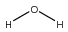
\includegraphics[width=2cm]{images/water} \end{wrapfigure}
Consider a water molecule. If you were describing it in terms of its structure to someone who understands the concept of atoms and bonds, but has no idea what the water molecule looks like, you might say:

\begin{quote}
	A water molecule contains an oxygen that is connected by single bonds to two hydrogen atoms.
\end{quote}

To describe the atoms in the grand scheme of the water molecule, you might say:

\begin{quote}
	A \qte{water oxygen} is an oxygen atom that is connected to two hydrogen atoms $via$ single bonds.
\end{quote}

...and...

\begin{quote}
	A \qte{water hydrogen} is a hydrogen that is connected $via$ a single bond to an oxygen atom, which is also connected by a single bond to another hydrogen atom.
\end{quote}

The extra information regarding the second hydrogen is necessary because otherwise we could apply the description of the \qte{water hydrogen} to the hydrogen in any alcohol group as well. Similarly, we might mistake the oxygen in the hydroxonium ion as being a \qte{water oxygen}, when in fact it is quite different. We should extend the description in this case to:

\begin{quote}
	A \qte{water oxygen} is an oxygen atom that is connected to two hydrogen atoms $via$ single bonds, and nothing else.
\end{quote}

An atom description in \progname{} is a string of comma-separated commands that explains this kind of criteria. So, to tell the program how to recognise a water oxygen and a water hydrogen, we could use the following type descriptions:\footnote{This and all following type descriptions are written in the proper forcefield input style (see section XXX). Briefly, the line consts of a unique type id number, a type name, the element symbol, and then the type description in double-quotes. Comments have also been added to describe the types.}


\begin{verbatim}
    1	OW	O	"nbonds=2,-H,-H"			# Water oxygen
    2	HW	H	"-O(nbonds=2,-H,-H)"			# Water hydrogen
\end{verbatim}

	
\progname{} reads this literally as \dqte{A water oxygen has exactly two bonds AND is bound to a hydrogen AND another hydrogen} and \dqte{A water hydrogen is bound to an oxygen that; has two bonds to it, is bound to a hydrogen, and is bound to another hydrogen}. The \qte{--X} is short-hand for saying \qte{is bound to X}, while the bracketed part after \qte{--O} in the water hydrogen description describes the required local environment of the attached oxygen. Using brackets to describe more fully the attached atoms is a crucial part of atom typing, and may be used to arbitrary depth (so, for example, we could add a bracketed description to the hydrogen atoms as well, if there was anything left to describe). If necessary, descriptions can be written that uniquely describe every single atom in a complex molecule by specifying completely all other connections within the molecule. This should not be needed for normal use, however, and short descriptions of atom environment up to first or second neighbours will usually suffice.\\


\subsection{Example 2 -- 3-hydroxypropanoic acid}
\index{typing examples}

\begin{wrapfigure}[]{l}[0em]{4.1cm} 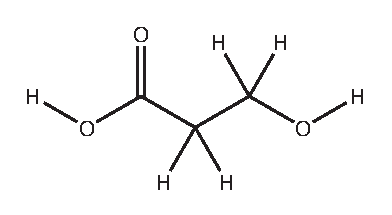
\includegraphics[width=4cm]{images/propanoic} \end{wrapfigure}
Assuming that the OH group in the carboxylic acid functionalisation will have different forcefield parameters to the primary alcohol at the other end of the molecule, here we must describe the first and second neighbours of the oxygen atoms to differentiate them. \\

To begin, we can describe the carbon atoms as either two or three different types -- either methylene/carboxylic acid, or carboxylic acid/adjacent to a carboxylic acid/adjacent to alcohol. For both, we only need describe the first neighbours of the atoms. For the first:

\begin{verbatim}
    3	C(H2)	C	"nbonds=4,-H,-H,-C"			# Methylene Carbon
    4	C_cbx	C	"nbonds=3,-O(bond=double),-O,-C"	# Carboxylic Acid C
\end{verbatim}

Note the ordering of the oxygen connections for the carboxylic acid carbon, where the most qualified carbon is listed first. This is to stop the doubly-bound oxygen being used to match \qte{--O}, subsequently preventing a successful match. \\

Where all three carbons need to be identified separately, we may write:

\begin{verbatim}
    5	C(OH)	C	"nbonds=4,-H,-H,-C,-O"			# CH2 adjacent to OH
    6	C(COOH)	C	"nbonds=4,-H,-H,-C,-C"			# CH2 adjacent to COOH
    7	C_cbx	C	"nbonds=3,-O(bond=double),-O,-C"	# Carboxylic Acid C
\end{verbatim}

Let us now assume that the hydrogens within the alcohol and carboxylic acid groups must also be seen as different types. In this case, the second neighbours of the atoms must be considered:

\begin{verbatim}
    8	HO	H	"-O(-C(-H,-H))"				# Alcoholic H
    9	H_cbx	H	"-O(-C(-O(bond=double)))"		# Carboxylic acid H
\end{verbatim}

The assignment is thus based entirely on the nature of the carbon atom to which the OH group is bound since this is the next available source of connectivity information. The determination of the three different oxygen atoms is similar:

\begin{verbatim}
    10	OH	O	"-H,-C(-H,-H)"				# Alcoholic O
    11	O_cbx	O	"-C(-O(-H))"				# Carboxylic acid =O
    12	OH_cbx	O	"-H,-C(-O(bond=double))"		# Carboxylic acid O(H)
\end{verbatim}

Of course, we could just have specified \dqte{nbonds=1} for the doubly-bound oxygen of the carboxylic acid group, but that wouldn't be very instructive, would it? 


\subsection{Example 3 -- $N$,$N$,2,5-tetramethylpyridin-4-amine}
\index{typing examples}

\begin{wrapfigure}[]{l}[0em]{3.1cm} 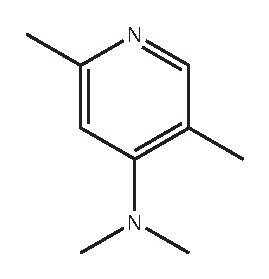
\includegraphics[width=3cm]{images/aromatic} \end{wrapfigure}
Ah, now here we have a proper problem! An asymmetric substituted pyridine. Lets assume that we need to distinguish between every non-hydrogen atom  -- we'll skip describing the hydrogen atoms for now, but note that this is most easily achieved by specifying directly the atomtype that the H is bound to (see later on). Let's start with the pyridine nitrogen. We basically need to say that its in a 6-membered aromatic ring:

\begin{verbatim}
    13	N_py	N	"ring(size=6,aromatic)"			# Pyridine N
\end{verbatim}

XXX

\section{Command Reference}
\label{sec:typingcommands}
\index{typing commands}

All type descriptions in files should be enclosed in double-quotes to prevent delimited parsing of strings. Commands may be separated by spaces or commas, but type descriptions may not span more than one line.

'-' (bound to)
Specifies a connection to another element, but not the exact type of the connection itself (i.e. the bond type, which may be specified with the \qte{bond} keyword in brackets after the element specifier). Immediately following the \qte{--} should be either an element symbol or a type id (the latter must be preceeded by a distinguishing \qte{\$}). Lists of the elements/type ids/type names may be given in square brackets, separated by commas or spaces, allowing multiple possibilities for matching the connection.

Examples:



bond, sp2, sp3, sp, unbound, geometry, ring (size)


XXX Repetition of descriptions - water example above. The dollar sign.

XXX Type scoring

XXX Art of type writing

XXX Order of atom descriptions



\chapter{Forcefields}

\section{File Format}
\label{sec:ffformat}
\index{forcefields!file format}

\section{Functional Forms}
\label{sec:ffforms}
\index{forcefields!functional forms}

\chapter{Filters Handbook}
\label{sec:filterhandbook}

\index{filters|(}
Filters are essentially just a series of text commands describing the format and structure of data in an arbitrary file. Plug-ins, if you like. While this might seem needlessly complex and a lot of extra work, for a little effort your (personal or enforced) favourite formats can be added to the program. The reward is a set of coordinates that can be thrown straight in to your code of choice. No support for writing out commands relevant to the running of calculations is provided, for three principal reasons:

\begin{enumerate}
	\item Input to codes is complicated, and I don't want to spend my evenings putting down endless combo boxes and spin buttons to cater for every basis set / method / obscure sub-option available.
	\item Putting commands in is best left for the user to do by hand, since there's no better way to learn the ins and outs of a code than to write commands, make mistakes, and be forced into the manual.
	\item The focus of \progname{} is on generating coordinates, pure and simple.
\end{enumerate}

But enough ranting! A filter contains (in order to be useful) sets of commands which describe how a file should be imported or exported from the program, and encompasses model files, forcefields, and trajectory files. However, different filters for the same file type may be provided if necessary, each performing a slightly different set of import or export commands (if it is convenient not do to so within a single filter), and all will appear in the drop-down list of filters in file dialogs within the program. Note that in batch, command-line, or scripting mode, filters are either selected automatically based on the filename, extension, or contents, or picked by matching only the associated nickname. In the former case, the first filter that matches the extension is used.\\

Filters are stored in one of two locations -- in a stock common to all users (as determined by the --prefix variable, or in the default location), and in \$HOME/.aten/filters. In both locations the filters read in by the program must be listed in the 'index' file -- if you create your own, you must add them to the index file for them to be loaded in on startup.\\

Read on and discover how to enable input / output of \qte{stuff} as you see fit. The following sections discuss the different aspects of filters and the types of file content that filters can be applied to, including examples. Although many of the commands are common to all of them, examples are good!

\subsection{Sections}
\index{filter!sections}
Commands to read / write different things are split up into sections within a filter file. You can specify as many filters as you like in any one file, each acting on a different set of models / forcefields / trajectories, etc., but it probably makes sense to have one file per model format where possible. All filter commands must be givin within one of these sections.

\begin{description}

	\item[importmodel\its]
	\index{filter commands!importmodel}
	Describes how to read model data from files, including atoms, cell and spacegroup data, and bonds.
	No variables are prepared by the command. Variables used after the command has completed:
	\begin{description}
		\item[$title$\its]
			Used to set the new title of the model.
		\item[$sg.group$ and $sg.setting$\its]
			Set the spacegroup and optionally the spacegroup setting so crystal packing can be performed.
	\end{description}

	\item[exportmodel\its]
	\index{filter commands!exportmodel}
	Write model data to files, including atoms, cell and spacegroup data, and bonds.\\
	Variables prepared by the command:
	\begin{description}
		\item[$title$\its]
			Title of the model.
		\item[$natoms$\its]
			Number of atoms in the model.
		\item[$cell.type$\its]
			Geometry of unit cell, one of \qte{none}, \qte{cubic}, \qte{orthorhombic}, or \qte{parallelepiped}.
		\item[$cell.x$, $cell.y$, $cell.z$\its]
			Lengths of the principal cell axes (if one is defined).
		\item[$cell.alpha$, $cell.beta$, $cell.gamma$\its]
			Angles between the principal cell axes (if one is defined).
		\item[$cell.xx$, $cell.xy$, $cell.xz$]
		\item[$cell.yx$, $cell.yy$, $cell.yz$]
		\item[$cell.zx$, $cell.zy$, $cell.zz$\its]
			Vector components of the unit cell matrix (if one is defined).
	\end{description}

	\item[trajectory]
	\index{filter commands!trajectory}
	Read trajectory files. Note that, since trajectory files often consist of a short descriptive header followed by frames listed end to end afterwards, 
	Variables prepared by the command:
	\begin{description}
		\item[$natoms$\its]
			Number of atoms in the model.
		\item[$cell.type$\its]
			Geometry of unit cell, one of \qte{none}, \qte{cubic}, \qte{orthorhombic}, or \qte{parallelepiped}.
	\end{description}

	\item[frame]
	\index{filter commands!frame}
	Read trajectory frame.\\
	Variables prepared by the command:
	\begin{description}
		\item[$natoms$\its]
			Number of atoms in the model.
		\item[$celltype$\its]
			Geometry of unit cell, one of \qte{none}, \qte{cubic}, \qte{orthorhombic}, or \qte{parallelepiped}.
	\end{description}

	\item[field]
	\index{filter commands!field}
	Write forcefield dsecription of current model.\\
	Variables set by the command:
	\begin{description}
		\item[$energyunit$\its]
			The current internal energy unit of the program, and hence the units used in the forcefield parameters.
		\item[$title$\its]
			Current title of the model.
		\item[$npatterns$\its]
			Number of different molecular species (pattern elements) in the model.
	\end{description}

\end{description}

\section{Recognising Files}
\label{sec:filterrecog}
\index{filters!recognising files}

Filters need a name. They are lonely creatures, and as such seek an identity. Although it can appear at more or less any point in the filter description, it usually makes most sense to name it early on. Consequently, the first line in most filters will be a short name describing what type of files the filter acts on:

\index{filter commands!name}
\begin{verbatim}
	name "ChikaanMol Coordinates File"
\end{verbatim}

This name will appear in the filter list of file dialogs in the GUI, and also in the program output when reading / writing files of the type. The next obvious question might be \dqte{How does the filter actually $recognise$ files of this type?} First off, there's the traditional way by filename extension:

\index{filter commands!extension}
\begin{verbatim}
	extension chik
\end{verbatim}

When files are being probed for their type, in the first instance the filename is examined and the extension (everything after the last \qte{.}) is compared to those defined in the filters. So, the example here would match all files ending with \qte{.ucf}. Sometimes one extension is not enough and there might be others that are used for the same type of file:

\begin{verbatim}
	extension "chik,egg,duk"
\end{verbatim}

Commas separate extensions, and the double-quotes are important to prevent \progname{} from interpreting the list as a list of arguments instead. Note that the comparison of filename extensions is case-insensitive, so \qte{.chk}, \qte{.EGG}, and \qte{.dUK} will all be matched by this filter.\\

Occasionally (and annoyingly) files have no extension at all, instead having short, fixed names. These exact names can be matched by the filter:

\index{filter commands!exact}
\begin{verbatim}
	exact config
\end{verbatim}

Exact filename matches are also case-insensitive, and lists of potential matches can be given, as before:

\begin{verbatim}
	exact "config,configuration,coordinates"
\end{verbatim}

Thirdly, the type of file can be matched by the contents of the file, and is probably of most use for the output of codes where the choice of filename for the results is entirely user-defined. For example, most codes print out a whole load of blurb and references at the very beginning, and usually searching for the program name within this region is enough:

\index{filter commands!within}
\begin{verbatim}
	within 10 "ChikaanMol version 2.2"
\end{verbatim}

This states that if the phrase \dqte{ChikaanMol version 2.2} can be found somewhere within the first 10 lines of the file, then the file is a match for this filter. One or more of the above criteria can be given, but it only takes a match with one of them to determine the type of file -- that is, they are not logically ANDed together.\\

All of the above is relevant to filters that import data. For exporting, \qte{exact} property is unused, but all others are relevant. When saving data without the aid of the GUI, the desired filter is specified through the use of a short nickname instead of by aspects of the filename, to avoid ambiguity.

\index{filter commands!nickname}
\begin{verbatim}
	nickname chikaan
\end{verbatim}

Used in an \qte{exportmodel} section, this allows one to specify the saving of data in the ubiquitous ChikaanMol coordinates format. In summary, use \qte{name}, \qte{extension}, and \qte{filter} in all sections, \qte{exact} (optionally) for filters that import data, and \qte{nickname} for filters that export data.

\section{Getting Data -- Format Strings}

So, now the file has been recognised, what happens next? We either read data in, or write data out. Enter \qte{format strings}. In nearly every way like FORMATs in Fortran and C/C++ $printf$ formats, these provide the interface to pass data between files and the program, and the sequence of commands is almost exactly like you would do in either of these programming languages. But for the uninitiated, don't panic! It's dead easy. Of course, in either language you use variables to store the data in the interim, and within filters this is no different. The basic (sub)processes in a filter are:

\begin{enumerate}
	\item Read data from a file.
	\item Split (parse) data into a number of variables.
	\item Tell \progname{} to act on the current values of variables.
\end{enumerate}

Variables thus form the bulk of the interface layer between numbers in a file, a filter to read them, and a program to use them (read--parse--act model). There are a handful of what you might call \qte{recognised} variables that mean something to the program in some way or other, but you are free to define your own at will to aid in the process of deconvoluting atomic data in awkward formats. See Section \ref{sec:variables} for a long waffle about variables in \progname{}. For now it is enough to know that variables are either generic character strings (converted to real or integer numbers as and when necessary) or special types such as, for example, references to atoms or patterns within the model. They are not declared at the beginning of the filter, instead being dynamically created and typed when they are required. All must begin with a \qte{\$} symbol to distinguish them from commands or plain text arguments to commands.

To demonstrate how these variables are used, lets assume that you have a file which is, for argument's sake, a coordinates file that has in it the following data:

\begin{verbatim}
Na      0.0     1.0     0.0
Cl      1.0     0.0     0.0
Na      0.0    -1.0     0.0
\end{verbatim}

Simply, elements and coordinates. Assuming that there's a filter command called \qte{readline} (there is) that reads in a line from a file and splits up the data on the line into a list of variables that you provide, if you were writing a command to describe one line of this data you would just say:

\begin{verbatim}
	readline "e r.x r.y r.z"
\end{verbatim}

The quoted part of the command is considered as the $format string$, and each element within it denotes a variable. After the command has completed, within the filter you can access the first item on the line that was read in by referencing the variable \qte{e}, the second with \qte{r.x}, and so on. These variables are all properties of an atom, but how do they actually become an atom? Well, these four are examples of so-called \qte{recognised} variables -- ones that the program looks for when storing or retrieving data (which depends on whether the filter itself is importing or exporting data). The command to create a new atom in the model we're currently reading in is \qte{addatom}, which, when run, looks for a number of specific variables from which to take data to set the properties of the new atom. In our example, it will find the variables \qte{e}, \qte{r.x}, \qte{r.y}, and \qte{r.z} and use them to set the element number and coordinates (it will also look for other variables which we have \textbf{not} set to any values, but won't complain when it can't find them). The situation is similar for other aspects of the model ($e.g.$ the unit cell), as well as for when we are writing data to a file instead of reading it -- the reverse process occurs, where we select an atom from the model (which sets the relevant variables) and then write out data using a format string containing these variables. \\

Lists of variables used or set by the various filter commands are given in the command reference in Section \ref{sec:filtercmds}. Also, see the chapter on variables (Section \ref{sec:variables}) for a full description and for details on how to specify the character length to read in, etc.


\subsection{Example -- XMol XYZ}
\label{sec:filterex1}
As always, things are best illustrated with an example. Take the XYZ format as popularised by XMol -- multiple models may be contained within a single file, each having a fixed structure with three basic data records:

\begin{enumerate}
  \item Number of atoms (1 line) -- Integer value specifying the number of atoms ($N$).
  \item Title (1 line) -- Long name or description of the system.
  \item Atom data ($N$ lines) -- Atom data, one per line, usually containing an aotomic element and its coordinates, but occasionally the atomic charge as well.
\end{enumerate}

For example:

\begin{verbatim}
3
Water
O     0.271   0.912   0.961    -0.8
H     0.978   1.244   1.295     0.4
H     0.126   0.149   1.307     0.4
\end{verbatim}

The corresponding filter can utilise the number of atoms provided in the file to read in the atom data, but this is not a general requirement since arbitrary loops can be defined to read in data until a certain point in the file (e.g. until a certain string is found, or simply until the end of the file is reached). The fully-specified filter (providing both import and export capabilities) for this type of file can be written as:

\begin{verbatim}
import
  name "XMol XYZ"
  extension xyz
  nickname xyz
  glob *.xyz
  readline "$natoms"
  readline "$title@100"
  repeat $n $natoms
    readline "$e $r.x $r.y $r.z $q"
    addatom
  end
  rebond
end
export
  name "XMol XYZ"
  glob *.xyz
  nickname xyz
  writeline "$natoms"
  writeline "$title"
  foratoms $i
    get $i
    writeline "$i.e@3 *@4 $i.r.x@12 $i.r.y@12 $i.r.z@12"
  end
end
\end{verbatim}

To begin, a descriptive name of the filter ({\it name "XMol XYZ"}), the common filename extension of the format ({\it extension xyz}), and a shell-style glob for the GUI file dialogs ({\it glob *.xyz}) are provided, giving the filetype description of the format. One post-load request is made, {\it rebond}, which indicates that bonds should be calculated for the model once all atoms have been loaded. Following this the list of commands to run when importing the file is given, beginning with the keyword {\it import}, and terminated with a matching {\it end} command. Recalling the structure of the xyz format, we expect to find the number of atoms on the first line, followed by the title of the model on the next, and then the atom data one per line after that. So, step-by-step the actions of the commands in this section are as follows:


\begin{description}
	\item[\texttt{readline "\$natoms"}\its]
		The {\it readline} command reads a line from the file and parses it according to some {\it format string}. Many commands rely on the use of format strings to interpret and store data. For now, we just appreciate that in this case the first item found on the line read from the file is placed in a variable named \qte{natoms}, which can then be used elsewhere.
	\item[\texttt{readline "\$title@100"}\its]
		Similar to the first command -- here we take the first 100 characters from the line and store it in a variable named \qte{title} -- here, \qte{title} is a variable name recognised internally by the program, and will be used to set the name of the model after import has finished.
	\item[\texttt{repeat \$n \$natoms}\its]
		The repeat loop runs a section of commands for a specified number of iterations (storing the value of the current iteration in a variable called \qte{n}). In this case the number of iterations is determined by the value of the variable {\it natoms} to allow us to read in the expected number of atomic data.
	\item[\texttt{readline "\$e \$r.x \$r.y \$r.z \$q"}\its]
		Here, the format string given to the readline command contains five parameters in line with the expected ordering of data in the XMol XYZ format. That is, the element symbol followed by the atomic coordinates, and then (possibly) an atomic charge.
	\item[\texttt{addatom}\its]
		At this point the current values of the temporary atom variables in the filter (in this example only the element, atomic coordinates, and atomic charge have been set) are saved in a new atom created in the model space.
	\item[\texttt{end}\its]
		Signals the end of the repeat loop.
	\item[\texttt{rebond}\its]
		Automatically calculate bonds between the atoms of the model.
\end{description}

XXX

\section{Filter Commands}
\label{sec:filtercmds}
\index{filter commands}

\subsection{File Description}
Definitions of the target file type and how to recognise it. Should be supplied in each filter section defined in a file.\\
\begin{description}

	\item[extension $list$\its]
	\index{filter commands!extension}
	Sets the filename extension that identifies files to be read / written by this filter.
	\begin{itemize}
		\item $e.g.$ \ttqte{extension xyz} means that files with extension \qte{xyz} will be recognised by this filter.
		\item $e.g.$ \ttqte{extension \dqte{xyz,abc,foo}} means that files with extensions \qte{xyz}, \qte{abc}, and \qte{foo} will be recognised by this filter.
	\end{itemize}

	\item[exact $list$\its]
	\index{filter commands!exact}
	Defines one or more exact filenames that identify files to be read / written by this filter.
	\begin{itemize}
		\item $e.g.$ \ttqte{exact coords} associates any file called \qte{coords} to this filter.
		\item $e.g.$ \ttqte{exact \dqte{results,output}} associates any files called \qte{results} or \qte{output} to this filter.
	\end{itemize}

	\item[filter $glob$\its]
	\index{filter commands!filter}
	Sets the file dialog filter extension to use in the GUI to the shell-style glob $glob$.
	\begin{itemize}
		\item $e.g.$ \ttqte{glob *.doc} filters any file matching \qte{*.doc} in the relevant GUI file selector dialogs.
	\end{itemize}

	\item[name $name$\its]
	\index{filter commands!name}
	Sets the long name of the filter to $name$, to be used as the filetype description of files identified by the filter.
	\begin{itemize}
		\item $e.g.$ \ttqte{name \dqte{SuperHartree Coordinates File}}.
	\end{itemize}

	\item[nickname $nick$\its]
	\index{filter commands!nickname}
	Sets the nickname of the filter to $nick$, which allows the filter to be identified in scripts.
	\begin{itemize}
		\item $e.g.$ \ttqte{nickname shart} sets the nickname of the filter to \qte{shart}.
	\end{itemize}

\end{description}


\subsection{Reading / Writing File Data}
Commands to parse data from files and variables.\\
\begin{description}

	\item[readline $format$\its]
	\index{filter commands!readline}
	Reads in the next line of the file (i.e., up to the carriage-return / newline marker) and splits up the data it finds into the variables specified in the $format$.
	\begin{itemize}
		\item $e.g.$ \ttqte{readline \dqte{\$n \$m \$title}} puts the first three whitespace-delimited items found on the next line in the file into the variables $n$, $m$, and $title$.
	\end{itemize}

	\item[writeline $format$\its]
	\index{filter commands!writeline}
	Constructs a string according to the $format$ given and writes it out to the file, appending a newline at the end.
	\begin{itemize}
		\item $e.g.$ \ttqte{writeline \dqte{NATOMS = \$natoms}} outputs a new line to the file, looking like \qte{NATOMS = 20}.
	\end{itemize}

\end{description}


\subsection{Storing Atom Data}
Create and set data for atoms in the model, and create bonds between them.\\
\begin{description}

	\item[addatom\its]
	\index{filter commands!addatom}
	The standard way of creating a new atom in the model. The command requires no arguments, and looks for variables set in the filter to store in the atom.
	\begin{itemize}
		\item $e.g.$ \ttqte{addatom}
	\end{itemize}

	Variables recognised by the command are:
	\begin{description}
		\item[$e$\its]
			Element symbol/Z/fftype of the atom
		\item[$r.x$, $r.y$, $r.z$\its]
			Coordinates of the atom.
		\item[$f.x$, $f.y$, $f.z$\its]
			Forces of the atom.
		\item[$v.x$, $v.y$, $v.z$\its]
			Velocities of the atom.
		\item[$q$\its]
			Charge on the atom
		\item[$id$\its]
			Numeric ID of the atom, used for bonding (see later).
	\end{description}
	If any of the variables cannot be found then the relevant properties are not set, otherwise the variables are reset afterwards ready for the next atom. Should the element variable $e$ be blank then the atom is set to element 0 (\qte{XX}). The numeric ID of the atom given by $id$ is a special case. If set it is stored as the atom's internal ID and can be referenced by the \qte{addbond} command, but as soon as loading has been finalised the atomic IDs are renumbered internally -- atom IDs set from the $id$ variable will not persist into the code.

	\item[addbond $id1$ $id2$ [$type$]\its]
	\index{filter commands!addbond}
	Bond two atoms with the specified IDs together with a singlne bond (if no bond type is specified) or of the type specified in $type$. The bond type may be given as a bond order (e.g. single = 1, double = 2, triple = 3) or as a string (\qte{single}, \qte{double}, or \qte{triple}). If the supplied $type$ is not recognised a single bond is used instead.
	\begin{itemize}
		\item $e.g.$ \ttqte{addbond 2 3} creates a single bond between atoms 2 and 3.
		\item $e.g.$ \ttqte{addbond 10 5 $btype$} creates a bond between atoms 10 and 5 whose type is held in the variable $btype$.
		\item $e.g.$ \ttqte{addbond 5 6 2} creates a double bond between atoms 5 and 6.
	\end{itemize}

	\item[createatoms $n$\its]
	\index{filter commands!createatoms}
	Creates a number $n$ of atoms at once in the model, whose properties may then be set individually (in any order) with the \qte{setatom} command. Atoms are all created initially with coordinates, forces, and velocities set to (0.0,0.0,0.0), a charge of 0.0, and with element type 0.
	\begin{itemize}
		\item $e.g.$ \ttqte{createatoms 52} creates 52 new atoms in the model.
		\item $e.g.$ \ttqte{createatoms $natoms$} creates new atoms in the model, the number depending on the value of the variable $natoms$.
	\end{itemize}

	\item[modeltemplate\its]
	\index{filter commands!modeltemplate}
	For use when reading trajectory frames, this command creates $n$ new atoms in the frame (where $n$ is the number of atoms currently in the parent model of the trajectory) and copies the element, colour, and rendering style data from the atoms in the parent model. Other properties such as the coordinates, velocities, and forces can then be defined with one of the \qte{set*} commands.
	\begin{itemize}
		\item $e.g.$ \ttqte{modeltemplate}.
	\end{itemize}

	\item[setatom $id$\its]
	\index{filter commands!setatom}
	Set the properties of the atom with the specified ID from variables set in the filter. The variables searched for are the same as for \qte{addatom}.
	\begin{itemize}
		\item $e.g.$ \ttqte{setatom 9} sets the data for atom ID 9 based on the values of variables already set in the filter.
		\item $e.g.$ \ttqte{setatom $i$} sets the data for atom $i$ based on the values of variables already set in the filter.
	\end{itemize}

	\item[setrx $id$ $value$\its]
	\index{filter commands!setrx}
	\item[setry $id$ $value$\its]
	\index{filter commands!setry}
	\item[setrz $id$ $value$\its]
	\index{filter commands!setrz}
	\item[setfx $id$ $value$\its]
	\index{filter commands!setfx}
	\item[setfy $id$ $value$\its]
	\index{filter commands!setfy}
	\item[setfz $id$ $value$\its]
	\index{filter commands!setfz}
	\item[setvx $id$ $value$\its]
	\index{filter commands!setvx}
	\item[setvy $id$ $value$\its]
	\index{filter commands!setvy}
	\item[setvz $id$ $value$\its]
	\index{filter commands!setvz}
	Set individual properties of the specified atom referenced by its ID. 
	\begin{itemize}
		\item $e.g.$ \ttqte{setrx 8 $posx$} sets the x-coordinate of atom 8 to the value of $posx$.
		\item $e.g.$ \ttqte{setfz 1 0.0} sets the z-component of the atomic forces of atom 1 to zero.
	\end{itemize}

\end{description}


\subsection{Loops}
Commands to perform plain repeat loops and loops over patterns, molecules, atoms, and forcefield terms. For loops that run over aspects of the model (e.g. atoms) the counter variable, elements of the control variable (e.g. the atom's name, coordinates etc.) may be accessed by referencing in the form $variable$.$property$. For example, the name and element symbol of an atom variable named \qte{i} may be retrieved with \qte{i.name} and \qte{i.symbol} respectively. Full lists of the variables set by the loops are given in the folowing list. All loop blocks must be terminated with an \qte{end} command.
\begin{description}

	\item[foratoms $var$ [$pattern$ [$molecule$]]\its]
	\index{filter commands!foratoms}
		Loop that runs over atoms in a model, pattern, or pattern molecule. The required variable $var$ is used to reference the current atom, while the second (optional) variable determines a specific pattern over which to loop (which may further be given a molecule number over which to restrict to). If only thne control variable is supplied the loop runs over all atoms in the current model.

		\begin{itemize}
			\item $e.g.$ to loop over all atoms $i$ in the model
			\begin{verbatim}
				foratoms $i
				...
				end
			\end{verbatim}

			\item $e.g.$ to loop over each atom $i$ in the representative molecule of a pattern referenced by $patternvar$
			\begin{verbatim}
				foratoms $atomnum $patternvar
				...
				end
			\end{verbatim}

			\item $e.g.$ to loop over all atoms $i$ in a specific molecule $m$ of pattern $p$
			\begin{verbatim}
				foratoms $i $p $m
				...
				end
			\end{verbatim}

			\item Properties available for the atom control variable are:
			\begin{description}
				\item[$symbol$\its]
					Element symbol of the atom.
				\item[$z$\its]
					Atomic number $Z$ of the atom.
				\item[$mass$\its]
					Atomic mass of the atom.
				\item[$name$\its]
					Element name of the atom.
				\item[$r.x$, $r.y$, $r.z$\its]
					Coordinates of the atom.
				\item[$f.x$, $f.y$, $f.z$\its]
					Forces of the atom.
				\item[$v.x$, $v.y$, $v.z$\its]
					Velocities of the atom.
				\item[$q$\its]
					Charge on the atom.
				\item[$fftype$\its]
					Forcefield type name associated to the atom (or \qte{???} if none).
				\item[$ffequiv$\its]
					Forcefield equivalent type name associated to the atom (or \qte{???} if none).
			\end{description}
		\end{itemize}

	\item[forffbonds $var$ $pattern$]
	\item[forffangles $var$ $pattern$]
	\item[forfftorsions $var$ $pattern$\its]
	\index{filter commands!forffbonds}
	\index{filter commands!forffangles}
	\index{filter commands!forfftorsions}
		Loops that run over the different forcefield elements of a pattern.
		\begin{itemize}
			\item $e.g.$ to loop over all patterns $p$ in the model
			\begin{verbatim}
				forpatterns $p
				...
				end
			\end{verbatim}

			Properties available for the control variable are:
			\begin{description}
				\item[$funcform$\its]
					Functional form of the term, corresponding to the keyword names in the original forcefield file (see Section XXX).
				\item[$id$\_$i$]
				\item[$id$\_$j$]
				\item[...\its]
					Molecule-relative ids of the atoms $i$, $j$, etc. involved in the term.
				\item[$param$\_$a$]
				\item[$param$\_$b$]
				\item[...\its]
					Parameters of the interaction, corresponding to the input order in the forcefield file (see Section XXX).
				\item[$type$\_$i$]
				\item[$type$\_$j$]
				\item[...\its]
					Forcefield types of the atoms $i$, $j$, etc. involved in the term.
			\end{description}
		\end{itemize}

	\item[formolecules $var$ $pattern$\its]
	\index{filter commands!formolecules}
		Specialised loop that runs over molecules in the patterns of a model, and so is of use when exporting data. The variable $var$ is used to store the current molecule number.
		\begin{itemize}
			\item $e.g.$ to loop over all molecules $m$ in a pattern $thispat$
			\begin{verbatim}
				formolecules $m $thispat
				...
				end
			\end{verbatim}
		\end{itemize}

	\item[forpatterns $var$\its]
	\index{filter commands!forpatterns}
		Specialised loop that runs over the patterns of a model, and so is of use when exporting data.
		\begin{itemize}
			\item $e.g.$ to loop over all patterns $p$ in the model
			\begin{verbatim}
				forpatterns $p
				...
				end
			\end{verbatim}

			Properties available for the pattern control variable are:
			\begin{description}
				\item[$name$\its]
					Name of the pattern.
				\item[$nmols$\its]
					Number of molecules encompassed by the pattern.
				\item[$nmolatoms$\its]
					Number of atoms per molecule.
				\item[$name$\its]
					Element name of the atom.
				\item[$nbonds$\its]
					Number of forcefield bond terms used in the expression for the pattern.
				\item[$nangles$\its]
					Number of forcefield angle terms used in the expression for the pattern.
				\item[$ntorsions$\its]
					Number of forcefield torsion terms used in the expression for the pattern.
			\end{description}
		\end{itemize}


	\item[repeat $var$ [$niter$]\its]
	\index{filter commands!repeat}
	Repeat commands up to the next \qte{end} for a number of iterations, storing loop iteration number in the variable $var$. $niter$ may either be a previously-initialised variable containing the number of iterations to perform, or an integer value. If $niter$ is not supplied the loop runs indefinitely and can only be terminated by the \qte{XXX} command or by reaching the end of the file.
	\begin{itemize}
		\item $e.g.$ \ttqte{repeat \$n} loops indefinitely, storing the current loop iteration in $n$.
		\item $e.g.$ \ttqte{repeat \$natoms 164} loops 164 times storing the current loop iteration in a variable $natoms$.
		\item $e.g.$ \ttqte{repeat \$atomno \$size} loops for the integer value of the $size$ variable, storing the current loop iteration in a variable $atomno$.
	\end{itemize}

	\item[while $var$ $test$ $value$\its]
	\index{filter commands!while}
	Repeats the commands in the following block while the condition provided evaluates to true (tested at the start of the block).
	\begin{itemize}
		\item $e.g.$ \ttqte{while element = Cl} loops while the variable $element$ contains a value of \qte{Cl}.
	\end{itemize}

\end{description}

\subsection{Storing a Unit Cell}
In particular, methods to set a handful of related variables for use in the filter, and to create / describe atoms from sets of known variables.\\
\begin{description}

	\item[setcellaxes\its]
	\index{filter commands!setcellaxes}
	Set the unit cell for the model / trajectory frame from cell length and angle variables already set in the filter. Lengths should be given in Angstroms and angles in degerees. The command expects to find values in:
	\begin{description}
		\item[$cell.a$]
		\item[$cell.b$]
		\item[$cell.c$\its]
			Lengths of the three cell axes.
		\item[$cell.alpha$]
		\item[$cell.beta$]
		\item[$cell.gamma$\its]
			Angles between cell axes.
	\end{description}

	\item[setcellvectors\its]
	\index{filter commands!setcellvectors}
	Set the unit cell for the model / trajectory frame from an axis matrix definition already set in the filter. Unit of length for axis definitions is \AA{}ngstroms. The command expects to find values in:
	\begin{description}
		\item[$cell.a.x$]
		\item[$cell.a.y$]
		\item[$cell.a.z$\its]
			Vector components of the cell's $A$ vector.
		\item[$cell.b.x$]
		\item[$cell.b.y$]
		\item[$cell.b.z$\its]
			Vector components of the cell's $B$ vector.
		\item[$cell.c.x$]
		\item[$cell.c.y$]
		\item[$cell.c.z$\its]
			Vector components of the cell's $C$ vector.
	\end{description}


\end{description}


\subsection{Testing Conditions}
Ways to perform tests on variables within the filter.\\
\begin{description}

	\item[if $var$ $test$ $value$\its]
	\index{filter commands!if}
	Tests the contents of the variable $var$ against either another variable named $value$, or a literal string $value$ (which it is assumed to be if a variable named $value$ does not currently exist) and executes the commands in the following block if the test is true. See Section \ref{sec:variables} for a list of tests and the way they are performed.
	\begin{itemize}
		\item $e.g.$ \ttqte{if \$natoms = 30} checks if the variable $natoms$ equals \qte{30}.
		\item $e.g.$ \ttqte{if \$style <> formatted} checks if the variable $style$ equals the string \qte{formatted}.
	\end{itemize}

	\item[else\its]
	\index{filter commands!else}
	Closes the command block of the most recent (as yet unterminated) \qte{if} or \qte{elseif} and begins another block, the contents of which will be executed if none of the preceeding tests evaluate to true.
	\begin{itemize}
		\item $e.g.$ \ttqte{else}
	\end{itemize}

	\item[elseif $var$ $test$ $value$\its]
	\index{filter commands!elseif}
	Closes the command block of the most recent (as yet unterminated) \qte{if} or \qte{elseif} and begins another \qte{if} block, the contents of which will be executed if its condition evaluates to true.
	\begin{itemize}
		\item $e.g.$ \ttqte{elseif \$natoms = 50} checks if the variable $natoms$ equals \qte{50}, executing the commands within the following block if this is so.
	\end{itemize}
	
	\item
		\begin{itemize}
			\item[$e.g.$]
			\begin{verbatim}
				if $name = alan
				  ...do something...
				elseif $name = bill
				  ...do something else...
				elseif $job = done
				  ...test on different variable...
				else
				  ...contingency plan...
				end
			\end{verbatim}
		\end{itemize}

\end{description}




By default, the atomic numbers of imported atoms are decoded from element symbols since this is the most common way in which they are represented in molecule file formats. Case is unimportant, so \qte{na}, \qte{Na}, and \qte{NA} will all be interpreted as atomic number 11 (sodium). When this proves to be inadequate, several extra options are available (set through the command line or file import dialog) allowing atomic numbers to be determined in different ways. The \qte{ff} option is particularly useful when loading in coordinate files which have atom names which do not necessarily correspond trivially to element information (e.g. DL\_POLY configurations) and where the atomic numbers of atoms cannot uniquely be determined from a simple comparison with element symbols. When decoding forcefield types, all forcefields which have been imported prior to model loading will be searched for the type names in the model file, and the atomic number set accordingly to the first exact match found.



\index{filters|)}
\chapter{Scriptors Handbook}
\index{scripts}
\index{command-line options!-s}
\index{command-line options!{-}{-}script}

The scripting and interactive modes of \progname{} allow most program procedures and actions to be controlled $via$ a series of text commands contained in a file or typed in directly. Files containing script commands are passed with the \qte{-s $file$} or \qte{{-}{-}script $file$} command-line options and are executed immediately following parsing of the commands in the file. Alternatively, a compound sequence of commands can be provided on the command line with the \qte{-c} or \qte{{-}{-}command} switches. As with filters, variables must be preceded with a \qte{\$}, so compound commands given on the command line must, for example, be enclosed with single-quotes to prevent the shell from expanding these variables itself.


\section{Inside the Script}
When performing a whole sequence of commands to perform actions without a visible workspace (i.e. the GUI), managing and using objects becomes more difficult. When dealing with models and forcefields in these cases, \progname{} does not use explicit references to different objects in order to accomplish tasks. For example, typically one might wish to:

\begin{itemize}
	\item Load a model $X$
	\item Edit $X$
	\item Edit $X$ a bit more
	\item Load a forcefield $Y$
	\item Associate a forcefield $Y$ with $X$
	\item Minimise a model $X$ with a forcefield $Y$
	\item Save a model $X$
	\item Go and have tea
\end{itemize}

Here, explicit references to the model $X$ and forcefield $Y$ are required every time they are used, which is verbose and rather incoherent with the same procedure when \qte{at the desk}. Instead, \progname{} uses the notion of $current$ objects ($i.e.$ those on the desk in front of you, as opposed to those waiting on the shelf behind you) which are the focus of all the commands, and means that no references to objects (models, forcefields etc.) are given to the commands, in the same spirit as the GUI where commands are implicitly executed on the model currently displayed. Obvious exceptions to this are those commands that provide methods to select other objects, thereby making them $current$.
Thus, whenever an object is created or loaded it becomes the current object of that type, receiving the effects of all commands relevant to it, and remains current (on the desk) until replaced (moved to the shelf) by another object of the same type being loaded, created, or selected. In the example above, all references to $X$ and $Y$ could then be removed since when the model and forcefield are loaded they become the current objects of their respective type, and the remaining commands work implicitly on these current objects.

Objects in scripts are referred to by names associated with them on their creation or loading, and may then be selected by reference to this name at a later stage.


\section{Quick Command Examples}
\index{scripts!examples}

\section{Command Reference}
\index{script commands}
%\subsection{Command \qte{translate}}
%\begin{description}
%	\item[]
%	\item[]
%\end{description}
%translate atom <dx> <dy> <dz> - Translate active atom
%translate selection <dx> <dy> <dz> - Translate selection

\subsection{Analysis}
\index{script commands!analysis}
Adds quantities / properties to be calculated to a pending joblist. The \qte{modelanalyse} and \qte{frameanalyse} subcommands calculate the pending properties in the joblist for the current model / frame and accumulate the data. The \qte{finalise} subcommand is used to normalise the calculated data and generate suitable averages from the accumulated data.\\
\begin{description}

	\item[finalise\its] Finalises the quantities in the pending jobs list, performing the necessary averages.
	\index{script commands!finalise}
	\begin{itemize}
		\item $e.g.$ \ttqte{finalise}.
	\end{itemize}

	\item[frameanalyse\its] Calculates all properties in the pending joblist for the current frame.
	\index{script commands!frameanalyse}
	\begin{itemize}
		\item $e.g.$ \ttqte{frameanalyse}.
	\end{itemize}

	\item[modelanalyse\its] Calculates all properties in the pending joblist for the current model.
	\index{script commands!modelanalyse}
	\begin{itemize}
		\item $e.g.$ \ttqte{modelanalyse}.
	\end{itemize}

	\item[pdens $name$ $site1$ $site2$ $spacing$ $npoints$\its] Adds a 3D probability distribution function $name$ to the pending jobs list for the model. Two sites must be specified, the first being the central species about which to calculate the distribution of the second. Axes must be specified for the first site with the \qte{setaxes} command. $spacing$ gives the spacing between grid points (assuming a cubic grid) while $npoints$ determines the number of grid points to use in each positive / negative direction.
	\index{script commands!pdens}
	\begin{itemize}
		\item $e.g.$ \ttqte{pdens mydens OHO centre 0.1 40} requests the calculation of a probability density called \qte{mydens} between the central site \qte{OHO} and the site \qte{centre}, with 40 gridpoints in each positive / negative direction with a spacing of 0.1 \AA{} (giving a grid extent of 4 \AA{} in each positive / negative direction, i.e. a grid of 81x81x81 points).
	\end{itemize}

	\item[printjobs\its] Prints a summary of the pending jobs list.
	\index{script commands!printjobs}
	\begin{itemize}
		\item $e.g.$ \ttqte{printjobs}.
	\end{itemize}

	\item[rdf $name$ $site1$ $site2$ $rmin$ $binwidth$ $nbins$\its] Adds a radial distribution function $name$ to the pending jobs list for the model. Two sites must be specified. The RDF is calculated over the distance range bounded by $rmin$ and $rmin + binwidth*nbins$.
	\index{script commands!rdf}
	\begin{itemize}
		\item $e.g.$ \ttqte{rdf cog N 0.0 0.1 200} calculates an RDF between the sites \qte{cog} and \qte{N} over the distance range 0.0 - 20.0 \AA{}.
	\end{itemize}

\end{description}

\subsection{Bonding}
\index{script commands!bonding}
Create bonds and perform automatic bonding operations.\\
\begin{description}

	\item[augment\its] Augments bonds in the current model.
	\index{script commands!augment}
	\begin{itemize}
		\item $e.g.$ \ttqte{augment}.
	\end{itemize}

	\item[rebond\its] Calculate bonding in the current model.
	\index{script commands!rebond}
	\begin{itemize}
		\item $e.g.$ \ttqte{rebond}.
	\end{itemize}

	\item[clearbonds\its] Delete all bonds in the current model.
	\index{script commands!clearbonds}
	\begin{itemize}
		\item $e.g.$ \ttqte{clearbonds}.
	\end{itemize}

	\item[bondpatterns\its] Calculate bonds within pattern molecules.
	\index{script commands!bondpatterns}
	\begin{itemize}
		\item $e.g.$ \ttqte{bondpatterns}.
	\end{itemize}

	\item[bondselection\its] Calculate bonds restricted to current atom selection.
	\index{script commands!bondselection}
	\begin{itemize}
		\item $e.g.$ \ttqte{bondselection}.
	\end{itemize}

	\item[bondtol $tol$\its] Adjust the bond calculation tolerance.
	\index{script commands!bondtol}
	\begin{itemize}
		\item $e.g.$ \ttqte{bondtol 1.20}.
	\end{itemize}

\end{description}


\subsection{Building}
\index{script commands!building}
Tools to build molecules from scratch, or finalise unfinished models. The drawing frame is represented as a set of three orthogonal vectors defining the reference coordinate system (set initially to the Cartesian axes) centred at an arbitrary origin (the pen position). Subsequent rotations operate on these coordinate axes.\\\\
\begin{description}

	\item[addhydrogen\its] Satisfy the valencies of all atoms in the current model by adding hydrogens to heavy atoms.
	\index{script commands!addhydrogen\its}
	\begin{itemize}
		\item $e.g.$ \ttqte{addhydrogen}.
	\end{itemize}

	\item[addatom $el$\its] Create a new atom of element $el$ at the current pen position.
	\index{script commands!addatom}
	\begin{itemize}
		\item $e.g.$ \ttqte{addatom N} places a nitrogen atom at the current pen coordinates.
	\end{itemize}

	\item[addchain $el$ [$bondtype$]\its] Create a new atom of element $el$ at the current pen position, bound to the last drawn atom with a single bond (or of type $bondtype$ if one was specified).
	\index{script commands!addchain}
	\begin{itemize}
		\item $e.g.$ \ttqte{addchain C} places a carbon atom at the current pen coordinates, and creates a single bond with the last drawn atom.
		\item $e.g.$ \ttqte{addchain O double} places an oxygen atom at the current pen coordinates, and creates a double bond with the last drawn atom.
	\end{itemize}

	\item[endchain\its] 'Ends the current chain (so that the next drawn 'chain' atom will not be bound to the last drawn atom).
	\index{script commands!endchain}
	\begin{itemize}
		\item $e.g.$ \ttqte{endchain}.
	\end{itemize}

	\item[locate $dx$ $dy$ $dz$\its] Sets the pen position to the coordinates specified (in Angstroms).
	\begin{itemize}
		\item $e.g.$ \ttqte{pen set 0.0 0.0 0.0} moves the pen back to the coordinate origin.
	\end{itemize}

	\item[move $dx$ $dy$ $dz$\its] Moves the pen position by the amounts specified (in Angstroms).
	\begin{itemize}
		\item $e.g.$ \ttqte{pen move 1.0 1.0 0.0} moves the pen +1 Angstrom in both the $x$ and $y$ directions.
	\end{itemize}

	\item[rotx $angle$\its] Rotates the reference coordinate system about the $x$ axis by $angle$ degrees.
	\begin{itemize}
		\item $e.g.$ \ttqte{pen rotx 90.0} rotates around the $x$ axis by 90$^\circ$.
	\end{itemize}

	\item[roty $angle$\its] Rotates the reference coordinate system about the $y$ axis by $angle$ degrees.
	\begin{itemize}
		\item $e.g.$ \ttqte{pen roty 45.0} rotates around the $y$ axis by 45$^\circ$.
	\end{itemize}

	\item[rotz $angle$\its] Rotates the reference coordinate system about the $z$ axis by $angle$ degrees.
	\begin{itemize}
		\item $e.g.$ \ttqte{pen rotz 109.5} rotates around the $z$ axis by 109.5$^\circ$.
	\end{itemize}

\end{description}


\subsection{Cell Editing}
\index{script commands!cell editing}
Unit cell actions.\\
\begin{description}

	\item[printcell\its] Prints the cell parameters of the current model.
	\index{script commands!printcell}
	\begin{itemize}
		\item $e.g.$ \ttqte{printcell}
	\end{itemize}

	\item[removecell\its] Clears any cell description (removes periodic boundary conditions) from the current model.
	\index{script commands!removecell}
	\begin{itemize}
		\item $e.g.$ \ttqte{removecell}
	\end{itemize}

	\item[scalecell $x$ $y$ $z$\its] Scale unit cell (and centres-of-geometry of molecules within it) by the scale factors $x$, $y$, and $z$.
	\index{script commands!scalecell}
	\begin{itemize}
		\item $e.g.$ \ttqte{scalecell 1.0 2.0 1.0} doubles the length of the $y$-axis of the system, stretching the positions of the molecules to reflect the new size. $x$ and $z$ axes remain unchanged.
	\end{itemize}

	\item[setcell $a$ $b$ $c$ $\alpha$ $\beta$ $\gamma$\its] Set cell lengths and angles of current model. This command will add a cell to a model currently without a unit cell specification.
	\index{script commands!setcell}
	\begin{itemize}
		\item $e.g.$ \ttqte{setcell 20.0 10.0 10.0 90.0 90.0 90.0} adds an orthorhombic cell with side lengths 20x10x10 \AA to the current model.
	\end{itemize}

\end{description}


\subsection{Charges}
\index{script commands!charges}
Assign partial charges to models, atoms, and patterns. Charges are specified in units of $e$.\\
\begin{description}

	\item[chargeatom $id$ $q$\its] Assign a charge of $q$ to atom $id$ in the current model.
	\index{script commands!chargeatom}
	\begin{itemize}
		\item $e.g.$ \ttqte{chargeatom 12 -0.2} assigns a charge of $-0.2$ to the twelfth atom.
	\end{itemize}

	\item[chargeff\its] Assigns charges to all atoms in the current model based on the forcefield associated to the model and the current types of the atoms.
	\index{script commands!chargeff}
	\begin{itemize}
		\item $e.g.$ \ttqte{chargeff}.
	\end{itemize}

	\item[chargefrommodel\its] Copies charges of all atoms in the current model to the atoms of the current trajectory frame.
	\index{script commands!chargefrommodel}
	\begin{itemize}
		\item $e.g.$ \ttqte{chargefrommodel}.
	\end{itemize}

	\item[chargepatom $id$ $q$\its] Assigns a charge of $q$ to atom $id$ in each molecule of the current pattern.
	\index{script commands!chargepatom}
	\begin{itemize}
		\item $e.g.$ \ttqte{chargepatom 3 0.1} assigns a charge of 0.1 to the third atom in each molecule of the current pattern.
	\end{itemize}

	\item[chargeselection $q$\its] Assigns a charge of $q$ to each selected atom in the current model.
	\index{script commands!chargeselection}
	\begin{itemize}
		\item $e.g.$ \ttqte{chargeselection 1.0} gives each atom in the current model's selection a charge of 1.0.
	\end{itemize}

	\item[chargetype $fftype$ $q$\its] Assigns a charge of $q$ to each atom that is of type $fftype$ in the current model.
	\index{script commands!chargetype}
	\begin{itemize}
		\item $e.g.$ \ttqte{chargetype OW -0.8} gives a charge of $-0.8$ to every atom that is of type \qte{OW}.
	\end{itemize}

	\item[clearcharges\its] Clears all charges in the current model, setting them to zero.
	\index{script commands!clearcharges}
	\begin{itemize}
		\item $e.g.$ \ttqte{clearcharges}.
	\end{itemize}

\end{description}


\subsection{Disordered Building}
\index{script commands!disordered building}
Build periodic disordered systems from individual components using Monte Carlo methods.\\
\begin{description}

	\item[addcomponent $model$ $nmols$ $name$\its] Specify that $nmols$ copies of the $model$ are to be added (or attempted to be added) during the build process. The component is referenced by the other commands from the provided $name$.
	\index{script commands!addcomponent}
	\begin{itemize}
		\item $e.g.$ \ttqte{addcomponent butane 300 bulk} requests that the \qte{butane} model should be entered into the list of components, referenced by the name \qte{bulk}, and that the disordered builder should attempt to create 300 copies of the model in the new system.
	\end{itemize}

	\item[setcellcentre $name$\its] Sets the coordinates of the centre of the region defined for component $name$ to the center of the cell.
	\index{script commands!setcellcentre}
	\begin{itemize}
		\item $e.g.$ \ttqte{setcellcentre propanol} sets the centre of the shape for \qte{propanol} to be the centre of the unit cell.
	\end{itemize}

	\item[setcenter $name$ $x$ $y$ $z$\its] Sets the coordinates of the centre of the region defined for component $name$.
	\index{script commands!setcenter}
	\begin{itemize}
		\item $e.g.$ \ttqte{setcenter propanol 5.0 7.0 6.0} sets the centre of the \qte{propanol} region to [5.0 7.0 6.0].
	\end{itemize}

	\item[setgeometry $name$ $x$ $y$ $z$ [$l$]\its] Sets the geometry of the region for component $name$. The $x$, $y$, and $z$ values determine the total extent of the region along each principal axis.
	\index{script commands!setgeometry}
	\begin{itemize}
		\item $e.g.$ \ttqte{setgeometry propanol 10.0 10.0 3.0} sets the geometry of the region for the \qte{propanol} component. For example, if the region was of type \qte{sphere} this would create an elongated ellipsoid.
	\end{itemize}

	\item[setoverlap $name$ $true|false$\its] Determines whether additions into the region are allowed to overlap with regions defined for other components. Default is true.
	\index{script commands!setoverlap}
	\begin{itemize}
		\item $e.g.$ \ttqte{setoverlap lysine false} restricts the \qte{lysine} component to the subspace of its defined region that does not overlap with any other region.
	\end{itemize}

	\item[printcomponents\its] Prints the current component list to be used in the disordered builder.
	\index{script commands!printcomponents}
	\begin{itemize}
		\item $e.g.$ \ttqte{printcomponents}.
	\end{itemize}

	\item[setshape $name$ $shape$\its] Sets the type of the allowed insertion region for the specified model (which should have already been \qte{add}ed). Valid $shape$s are \qte{cell}, \qte{cuboid}, \qte{spheroid}, and \qte{cylinder}.
	\index{script commands!setshape}
	\begin{itemize}
		\item $e.g.$ \ttqte{setshape propanol sphere} restricts the component \qte{propanol} to a spherical region of the cell.
	\end{itemize}

	\item[disorder $ncycle$\its] Start the disordered builder, requesting $ncycle$ cycles of Monte Carlo moves.
	\index{script commands!disorder}
	\begin{itemize}
		\item $e.g.$ \ttqte{disorder 50} runs 50 cycles of the disordered builder.
	\end{itemize}

	\item[vdwscale $scale$\its] Sets the scaling factor for VDW radii to use in the disordered builder.
	\index{script commands!vdwscale}
	\begin{itemize}
		\item $e.g.$ \ttqte{vdwscale 0.75} scales all VDW radii by 0.75 in the calculation.
	\end{itemize}

\end{description}

\subsection{Energy Calculation}
\index{script commands!energy calculation}
Calculate energies for models and trajectory frames. All printing commands refer to the last energy calculated for either the model or a trajectory frame.\\
\begin{description}

	\item[frameenergy\its] Calculate energy of the current frame of the trajectory associated with the current model.
	\index{script commands!frameenergy}
	\begin{itemize}
		\item $e.g.$ \ttqte{frameenergy}.
	\end{itemize}

	\item[modelenergy\its] Calculate the energy of the current model, which can then be printed out (in whole or by parts) by the other subcommands.
	\index{script commands!modelenergy}
	\begin{itemize}
		\item $e.g.$ \ttqte{modelenergy}.
	\end{itemize}

	\item[printelec\its] Prints out the electrostatic energy decomposition matrix.
	\index{script commands!printelec}
	\begin{itemize}
		\item $e.g.$ \ttqte{printelec}.
	\end{itemize}

	\item[printewald\its] Prints the components of the Ewald sum energy.
	\index{script commands!printewald}
	\begin{itemize}
		\item $e.g.$ \ttqte{printewald}.
	\end{itemize}

	\item[printinter\its] Prints out the total inter-pattern energy decomposition matrix.
	\index{script commands!printinter}
	\begin{itemize}
		\item $e.g.$ \ttqte{printinter}.
	\end{itemize}

	\item[printintra\its] Prints out the total intramolecular energy decomposition matrix.
	\index{script commands!printintra}
	\begin{itemize}
		\item $e.g.$ \ttqte{printintra}.
	\end{itemize}

	\item[printenergy\its] Prints the elements of the calculated energy in a list.
	\index{script commands!printenergy}
	\begin{itemize}
		\item $e.g.$ \ttqte{printenergy}.
	\end{itemize}

	\item[printsummary\its] Print out a one-line summary of the calculated energy.
	\index{script commands!printsummary}
	\begin{itemize}
		\item $e.g.$ \ttqte{printsummary}.
	\end{itemize}

	\item[printvdw\its] Prints out the VDW energy decomposition matrix.
	\begin{itemize}
		\item $e.g.$ \ttqte{printvdw}.
	\end{itemize}

\end{description}

\subsection{Expression}
\index{script commands!expression}
Manage the energy setup and forcefield expression.\\
\begin{description}

	\item[createexpression\its] Creates a suitable energy description for the current model.
	\index{script commands!createexpression}
	\begin{itemize}
		\item $e.g.$ \ttqte{createexpression}.
	\end{itemize}

	\item[ecut $distance$\its] Sets the electrostatic cutoff (for Coulomb sum and real-space part of Ewald sum) to $distance$.
	\index{script commands!ecut}
	\begin{itemize}
		\item $e.g.$ \ttqte{ecut 14.5} sets the electrostatic cutoff distance to 14.5 \AA.
	\end{itemize}

	\item[elec $style ...$\its] Selects the method of calculation for electrostatic energy and forces (default is \qte{none}).
	\index{script commands!elec}
	\begin{itemize}
		\item \ttqte{elec none} turns off electrostatics.
		\item \ttqte{elec coulomb} uses the coulomb sum.
		\item \ttqte{elec ewald $alpha$ $kx$ $ky$ $kz$} selects the Ewald sum with convergence parameter $alpha$ and $k$-vectors specified.
		\item $e.g.$ \ttqte{elec ewald 0.2 9 9 9}.
		\item \ttqte{elec ewaldauto $precision$} selects Ewald sum with automatic parameter generation governed by precision specified.
		\item $e.g.$ \ttqte{elec ewaldauto 5.0e-6} auto-calculates $alpha$ and $kmax$ with XXX precision of 5.0e-6.
	\end{itemize}

	\item[intra $on|off$\its] Controls calculation of intramolecular terms in energy / force calculations (on by default).
	\index{script commands!intra}
	\begin{itemize}
		\item $e.g.$ \ttqte{intra off} turns intramolecular energy / force calculation off.
	\end{itemize}

	\item[printexpression\its] Prints the current expression setup.
	\index{script commands!printexpression}
	\begin{itemize}
		\item $e.g.$ \ttqte{printexpression}
	\end{itemize}

	\item[vcut $distance$\its] Sets the van der Waals cutoff to $distance$.
	\index{script commands!vcut}
	\begin{itemize}
		\item $e.g.$ \ttqte{vcut 20.0} sets van der Waals cutoff distance to 20.0 \AA.
	\end{itemize}

	\item[vdw $on|off$\its] Controls calculation of van der Waals terms in energy / force calculations (on by default).
	\index{script commands!vdw}
	\begin{itemize}
		\item $e.g.$ \ttqte{vdw off} turns van der Waals energy / force calculation off.
	\end{itemize}

\end{description}

\subsection{Forcefields}
\index{script commands!forcefields}
Basic forcefield management.\\
\begin{description}

	\item[ffmodel\its] Associates current forcefield to the current model.
	\index{script commands!ffmodel\its}
	\begin{itemize}
		\item $e.g.$ \ttqte{ffmodel}.
	\end{itemize}

	\item[ffpattern\its] Associates current forcefield to the current pattern.
	\index{script commands!ffpattern}
	\begin{itemize}
		\item $e.g.$ \ttqte{ffpattern}.
	\end{itemize}

	\item[ffpatternid $id$\its] 
	\index{script commands!ffpatternid}
	\begin{itemize}
		\item $e.g.$ \ttqte{ffpatternid 3}.
	\end{itemize}

	\item[loadff $file$ $name$\its] Load a forcefield from $file$ and reference it by $name$. Becomes the current forcefield.
	\index{script commands!loadff}
	\begin{itemize}
		\item $e.g.$ \ttqte{loadff /home/foo/complex.ff waterff} loads a forcefield called \qte{complex.ff} and names it \qte{waterff}.
	\end{itemize}

	\item[selectff $name$\its] Selects the forcefield $name$ and makes it the current forcefield. If a forcefield of that name is not loaded an error is returned.
	\index{script commands!selectff}
	\begin{itemize}
		\item $e.g.$ \ttqte{selectff organicff} makes the forcefield \qte{organicff} current.
	\end{itemize}

\end{description}


\subsection{Forces}
\index{script commands!forces}
Calculate forces for models and trajectory frames.\\
\begin{description}

	\item[frameforces\its] Calculate the atomic forces of the current frame of the trajectory associated with the current model.
	\index{script commands!frameforces}
	\begin{itemize}
		\item $e.g.$ \ttqte{frameforces}.
	\end{itemize}

	\item[modelforces\its] Calculate the atomic forces of the current model.
	\index{script commands!modelforces}
	\begin{itemize}
		\item $e.g.$ \ttqte{modelforces}.
	\end{itemize}

	\item[printforces\its] Print out the forces of the current model.
	\index{script commands!printforces}
	\begin{itemize}
		\item $e.g.$ \ttqte{printforces}.
	\end{itemize}

\end{description}

\subsection{Monte Carlo}
\index{script commands!mc}
Change parameters for Monte Carlo-based calculations. Energy values are given in the current working unit of energy in the program.\\
\begin{description}

	\item[mcaccept $move$ $emax$\its] Sets the energy difference $emax$ for the movetype $move$ above which moves will be rejected.
	\index{script commands!mcaccept}
	\begin{itemize}
		\item $e.g.$ \ttqte{mcaccept translate 0.0} requests that only translation moves that lower the overall energy will be accepted.
		\item $e.g.$ \ttqte{mcaccept insert 200.0} requests that insertion moves will be accepted provided the total energy does not rise more than 200.0 units.
	\end{itemize}

	\item[mcmaxstep $move$ $size$\its] Sets the maximal stepsize for the move type $move$.
	\index{script commands!mcmaxstep}
	\begin{itemize}
		\item $e.g.$ \ttqte{mcmaxstep translate 5.0} sets the maximum translation displacement to 5 \AA.
		\item $e.g.$ \ttqte{mcmaxstep rotate 30.0} sets the maximum rotation to 30$^\circ$.
	\end{itemize}

	\item[mcntrials $move$ $n$\its] Sets the number of times $n$ that the move type $move$ should be attempted in each cycle.
	\index{script commands!mcntrials}
	\begin{itemize}
		\item $e.g.$ \ttqte{mcntrials insert 50} requests that there will be 50 insertion attempts per cycle per molecule type.
	\end{itemize}

	\item[printmc\its] Prints the current Monte Carlo parameters.
	\index{script commands!printmc}
	\begin{itemize}
		\item $e.g.$ \ttqte{printmc}
	\end{itemize}

\end{description}


\subsection{Minimisation}
\index{script commands!minimisation}
Perform geometry minimisation on models.\\
\begin{description}

	\item[converge $econv$ $fconv$\its] Sets the convergence criteria of the minimisation methods. Energy and force convergence values are given in the current working unit of energy in the program.
	\index{script commands!converge}
	\begin{itemize}
		\item $e.g.$ \ttqte{converge 1e-6 1e-4} sets the energy and RMS force convergence criteria to 1x$10^{-6}$ and 1x$10^{-4}$ respectively.
	\end{itemize}

	\item[mcminimise $maxsteps$\its] Optimises the current model using a Monte Carlo minimisation method.
	\index{script commands!mcminimise}
	\begin{itemize}
		\item $e.g.$ \ttqte{mcminimise 20} runs a geometry optimisation for a maximum of 20 cycles.
	\end{itemize}

	\item[sdminimise $maxsteps$ $maxtrials$ $stepsize$\its] Optimises the current model using the Steepest Descent method.
	\index{script commands!sdminimise}
	\begin{itemize}
		\item $e.g.$ \ttqte{sdminimise 100 50 0.5} minimises the current model for a maximum of 100 Steepest Descent steps, with the maximum line trials per step set to 50, and the XXX
	\end{itemize}

\end{description}


\subsection{Models}
\index{script commands!models}
Basic model management.\\
\begin{description}{\setlength{\itemsep}{2em}}

	\item[listmodels\its] Lists all models currently available in the workspace.
	\index{script commands!listmodels}
	\begin{itemize}
		\item $e.g.$ \ttqte{listmodels}.
	\end{itemize}

	\item[loadmodel $file$ $name$\its] Load a model from $file$, referenced by $name$, which becomes the current model.
	\index{script commands!loadmodel}
	\begin{itemize}
		\item $e.g.$ \ttqte{loadmodel /home/foo/coords/test.xyz mymodel} loads a model called test.xyz and gives it the name \qte{mymodel}.
	\end{itemize}

	\item[newmodel $name$\its] Create a new model, referenced by $name$, which becomes the current model.
	\index{script commands!newmodel}
	\begin{itemize}
		\item $e.g.$ \ttqte{newmodel emptymodel} creats a new model called \qte{emptymodel} and makes it current.
	\end{itemize}

	\item[printmodel\its] Print out information on the current model and its atoms.
	\index{script commands!printmodel}
	\begin{itemize}
		\item $e.g.$ \ttqte{printmodel} outputs something like:
		\begin{verbatim}
			XXX Some crap here.
		\end{verbatim}
	\end{itemize}

	\item[savemodel $format$ $file$\its] Save the current model to $file$ in $format$.
	\index{script commands!savemodel}
	\begin{itemize}
		\item $e.g.$ \ttqte{savemodel xyz /home/foo/newcoords/test.config} saves the current model in \qte{xyz} format to the filename given.
	\end{itemize}

	\item[selectmodel $name$\its] Make $name$ the current model. If $name$ cannot be found an error is returned.
	\index{script commands!selectmodel}
	\begin{itemize}
		\item $e.g.$ \ttqte{selectmodel othermodel} makes the model called \qte{othermodel} current.
	\end{itemize}

\end{description}


\subsection{Patterns}
\index{script commands!patterns}
Automatically or manually create pattern descriptions for models.\\
\begin{description}

	\item[addpattern $nmols$ $natoms$ $name$\its] Add a new pattern node to the current model, spanning $nmols$ molecules of $natoms$ atoms each, and called $name$.
	\index{script commands!addpattern}
	\begin{itemize}
		\item $e.g.$ \ttqte{addpattern 100 3 water} creates a new pattern description of 100 molecules of 3 atoms each (i.e. 100 water molecules) in the current model.
	\end{itemize}

	\item[clearpatterns\its] Delete the pattern description of the current model.
	\index{script commands!clearpatterns}
	\begin{itemize}
		\item $e.g.$ \ttqte{clearpatterns}.
	\end{itemize}

	\item[createpatterns\its] Automatically detect and create the pattern description for the current model.
	\index{script commands!createpatterns}
	\begin{itemize}
		\item $e.g.$ \ttqte{createpatterns}.
	\end{itemize}

	\item[printpatterns\its] Prints out the current pattern description of the current model.
	\index{script commands!printpatterns}
	\begin{itemize}
		\item $e.g.$ \ttqte{printpatterns}.
	\end{itemize}

	\item[selectpattern $name$\its] Selects the pattern $name$ in the current model to be the current pattern. If the pattern cannot be found an error is returned.
	\index{script commands!selectpattern}
	\begin{itemize}
		\item $e.g.$ \ttqte{selectpattern formate} selects a pattern named \qte{formate}.
	\end{itemize}

\end{description}


\subsection{Selection}
\index{script commands!selection}
Select atoms or groups of atoms.\\
\begin{description}

	\item[invert\its] Inverts the selection of all atoms in the current model.
	\index{script commands!invert}
	\begin{itemize}
		\item $e.g.$ \ttqte{invert}.
	\end{itemize}

	\item[selectall\its] Select all atoms in the current model.
	\index{script commands!selectall}
	\begin{itemize}
		\item $e.g.$ \ttqte{selectall}.
	\end{itemize}

	\item[selectatom $id$\its] Select atom $id$ in the current model.
	\index{script commands!selectatom}
	\begin{itemize}
		\item $e.g.$ \ttqte{selectatom 45} selects the 45th atom.
	\end{itemize}

	\item[selectelement $el$\its] Select all atoms that are element $el$ in the current model.
	\index{script commands!selectelement}
	\begin{itemize}
		\item $e.g.$ \ttqte{selectelement Br} selects all bromine atoms.
	\end{itemize}

	\item[selectfftype $fftype$\its] Select all atoms with forcefield type $fftype$ in the current model.
	\index{script commands!selecttype}
	\begin{itemize}
		\item $e.g.$ \ttqte{selecttype CT} selects all atoms that are of type \qte{CT}.
	\end{itemize}

	\item[selectnone\its] Deselect all atoms in the current model.
	\index{script commands!selectnone}
	\begin{itemize}
		\item $e.g.$ \ttqte{selectnone}.
	\end{itemize}

	\item[selecttype $element$ $description$\its] Select atoms that are $element$ and match the type $description$ given.
	\index{script commands!selectatomtype}
	\begin{itemize}
		\item $e.g.$ \ttqte{selectatomtype C ''-H(n=2)''} selects all carbon atoms that are bound to two hydrogens.
	\end{itemize}

\end{description}


\subsection{Sites}
\index{script commands!sites}
Describe sites within molecules for use in analysis.\\
\begin{description}

	\item[addsite $name$ $pattern$ ``$atomlist$``\its] Creates a new site $name$ for the current model, based on the molecule of $pattern$, and placed at the geometric centre of the atom ids given in $atomlist$. If no atoms are given, the centre of geometry of all atoms is used. The new site becomes the current site.
	\index{script commands!addsite}
	\begin{itemize}
		\item $e.g.$ \ttqte{addsite watercentre h2o} adds a site called \qte{watercentre} based on the pattern called \qte{h2o} and located at the centre of geometry of all atoms.
		\item $e.g.$ \ttqte{addsite oxy methanol 5} adds a site called \qte{oxy} based on the pattern called \qte{methanol} and located at the fifth atom in each molecule.
	\end{itemize}

	\item[printsites\its] Prints the list of sites defined for the current model.
	\index{script commands!printsites}
	\begin{itemize}
		\item $e.g.$ \ttqte{printsites}.
	\end{itemize}

	\item[selectsite $name$\its] Selects (makes current) the site referenced by $name$. If the site cannot be found an error is returned.
	\index{script commands!selectsite}
	\begin{itemize}
		\item $e.g.$ \ttqte{selectsite carb1} makes the site \qte{carb1} the current site.
	\end{itemize}

	\item[setaxes \qte{$atomlist$} \qte{$atomlist$}\its] Sets the local x (first set of atom ids) and y (second set of atom ids) axes for the current site. Each of the two axes is constructed by taking the vector from the site centre (defined by the list of atoms given to \qte{addsite}) and the geometric centre of the list of atoms provided here. The y axis is orthogonalised with respect to the x axis and the z axis constructed from the cross product of the two orthogonal vectors.
	\index{script commands!setaxes}
	\begin{itemize}
		\item $e.g.$ \ttqte{setaxes '1,2' '6'} sets the x axis definition of the current site to be the vector between the site centre and the average position of the first two atoms, and the y axis definition to be the vector between the site centre and the position of the sixth atom.
	\end{itemize}

\end{description}


\subsection{Options}
\index{script commands!options}
Control miscellaneous aspects of the program and its behaviour. Boolean arguments are specified as on/off, but may also take the form yes/no or true/false.\\
\begin{description}

	\item[atomdetail $i$\its]
		Sets the number of slices / stacks to use in the rendering of polygonal spheres.
	
	\item[bonddetail $i$\its]
		Sets the number of slices / stacks to use in the rendering of polygonal tubes.

	\item[densityunits $units$\its] Set the density units to use in output. See Section \ref{sec:prefs} for a list of possibilities.
	\index{script commands!densityunits}
	\begin{itemize}
		\item $e.g.$ \ttqte{densityunits gpercm3} gives densities in g cm$^{-3}$.
	\end{itemize}

	\item[energyunits $units$\its] Set the unit of energy to use in output. See Section \ref{sec:prefs} for a list of possibilities.
	\index{script commands!energyunits}
	\begin{itemize}
		\item $e.g.$ \ttqte{energyunits kcal} shows energy values in units of kcal mol$^{-1}$.
	\end{itemize}

	\item[gl $option$ $on|off$\its]
	%linealias|polyalias|backcull|fog]
		Enables various OpenGL features (all are disabled by default).
		\begin{description}
			\item[linealias] Enable line aliasing
			\item[polyalias] Enable polygon aliasing (Note - has odd effects in the current version)
			\item[backcull] Enable backface culling of polygons
			\item[fog] Enable depth cueing.
		\end{description}
	
	\item[key $button$ $action$\its]
		Sets the action of the modifier keys that change normal mouse actions into their alternatives. Valid modifier keys are \qte{shift}, \qte{ctrl}, and \qte{alt}. Valid actions are:
			\begin{description}
				\item[zrotate] Changes a normal $x$/$y$ rotation action into rotation about the world $z$-axis
				\item[transform] Performs rotations and translations on the model coordinates rather than the view (i.e. a {it translate} action will translate the selected model coordinates instead of the camera)
				\item[none] The key does nothing. At all.
			\end{description}

	\item[mouse $button$ $action$\its]
		Sets the action of the specified button. Valid $button$s are \qte{left}, \qte{middle}, and \qte{right}. Valid actions are:
			\begin{description}
				\item[none] Gives you a useless button
				\item[rotate] Free rotation of the model around the $x$ and $y$ axes
				\item[zrotate] Rotation of the model around the $z$ axis
				\item[translate] Shifts the model in the world $xy$ plane of the current view (i.e. in the plane of the screen)
				\item[zoom] Moves the model back and forth along the local z-axis (into the screen) on moving the mouse up and down respectively
				\item[interact] Performs almost every other action including selection, drawing etc.
			\end{description}
	
	\item[movestyle $viewstyle$\its]
		The drawing style to use for models when rotating, manipulating etc. For those with lots of atoms and mid-range graphics cards, {\it stick} is probably a sensible option.
	

	\item[radius $viewstyle$ $f$]
		Sets the standard atom radius to use in the different drawing styles, although the effect of the radius differs between styles. For \qte{tube} and \qte{sphere} $f$ defines the actual radius (and consequently the selection hotspot radius) of on-screen atoms in Angstroms. For the \qte{stick} style it determines only the hotspot radius of the atoms. The \qte{scaled} style uses $f$ as a scaling factor applied to the elemental radii defined in the elements definition file \qte{elements.dat}.

	\item[shininess $i$\its]
		Sets the shininess of materials. $i$ should be in the range 0-255.
	
	\item[show $object$ $on|off$\its]
		Sets the visibility of objects in the rendering canvas. Valid $object$s are:
		\begin{description}
			\item[atoms] Atoms and bonds within the model
			\item[cell] The unit cell
			\item[cellaxes] Cell axis arrows at the origin of the unit cell
			\item[cellrepeat] Repeat units of the unit cell
			\item[forcearrows] Atomic force arrows
			\item[globe] The rotation globe displaying the cartesian axes
			\item[labels] Atomic labels
			\item[measurements] Geometry measurements
			\item[regions] Regions for components in the disordered builder
		\end{description}

	\item[style $viewstyle$\its]
		The default drawing style to use for all new models. Valid $viewstyle$s are \qte{stick}, \qte{tube}, \qte{sphere}, and \qte{scaled}.

\end{description}


\subsection{Trajectories}
\index{script commands!trajectories}
Open and select frames from the trajectory file associated to the current model.\\
\begin{description}

	\item[firstframe\its] Select the first frame from trajectory of current model.
	\index{script commands!firstframe}
	\begin{itemize}
		\item $e.g.$ \ttqte{firstframe}.
	\end{itemize}

	\item[lastframe\its] Select last frame in trajectory of current model.
	\index{script commands!lastframe\its}
	\begin{itemize}
		\item $e.g.$ \ttqte{lastframe\its}.
	\end{itemize}

	\item[loadtrajectory $file$\its] Associate trajectory in $file$ with current model.
	\index{script commands!loadtrajectory}
	\begin{itemize}
		\item $e.g.$ \ttqte{loadtrajectory /home/foo/md/water.HISf} opens and associated the DL\_POLY trajectory file \qte{water.HISf} with the current model.
	\end{itemize}

	\item[nextframe\its] Select next frame from trajectory of current model.
	\index{script commands!nextframe\its}
	\begin{itemize}
		\item $e.g.$ \ttqte{nextframe}.
	\end{itemize}

	\item[prevframe\its] Select the previous frame from the trajectory of the current model.
	\index{script commands!prevframe\its}
	\begin{itemize}
		\item $e.g.$ \ttqte{prevframe}.
	\end{itemize}

\end{description}


\chapter{Command Line Options}
\label{sec:cli}
\index{command-line options}
\index{cli}


\begin{optlist}{Import}

	\item[-f $file$, {-}{-}ff $file$]
	\index{command-line options!-f}
	\index{command-line options!{-}{-}ff}
		Loads the specified forcefield file before any models specified on the command line.

	\item[{-}{-}fold, {-}{-}nofold\its]
	\index{command-line options!{-}{-}fold}
	\index{command-line options!{-}{-}nofold}
		Force or prevent initial folding of atoms to within the boundaries of the unit cell (if one is present) in loaded models, overriding filter directives.
	
	\item[{-}{-}pack, {-}{-}nopack\its]
	\index{command-line options!{-}{-}pack}
	\index{command-line options!{-}{-}nopack}
		Force or prevent generation of symmetry-equivalent atoms from spacegroup information in loaded models, overriding filter directives.
	
	\item[{-}{-}bond, {-}{-}nobond\its]
	\index{command-line options!{-}{-}bond}
	\index{command-line options!{-}{-}nobond}
		Force or prevent (re)calculation of bonding in loaded models, overriding filter directives.
	
	\item[{-}{-}centre, {-}{-}nocentre\its]
	\index{command-line options!{-}{-}centre}
	\index{command-line options!{-}{-}nocentre}
		Prevent translation of non-periodic models’ centre-of-geometry to the origin, overriding filter directives.
	
	\item[-b, {-}{-}bohr\its]
	\index{command-line options!{-}{-}bohr}
		Specifies that the unit of length used in loaded models is Bohr rather than Angstrom, and should be converted to the latter.

\end{optlist}


\begin{optlist}{Output / Debugging}

	\item[-d, {-}{-}debug\its]
	\index{command-line options!-d}
	\index{command-line options!{-}{-}debug}
		Enables debugging of subroutine calls.
	
	\item[{-}{-}debugtyping\its]
	\index{command-line options!{-}{-}debugtyping}
		Enables output from the atom typing routines.
	
	\item[{-}{-}debugfilters\its]
	\index{command-line options!{-}{-}debugfilters}
		Enables output from the filter routines.
	
	\item[{-}{-}debugall\its]
	\index{command-line options!{-}{-}debugall}
		Enables output from the most all routines.

	\item[{-}{-}debugparse\its]
	\index{command-line options!{-}{-}debugparse}
		Enables output from the file parsing routines.
		
	\item[{-}{-}verbose\its]
	\index{command-line options!{-}{-}verbose}
		Switch on verbose reporting of program actions.

\end{optlist}

\begin{optlist}{Modes}

	\item[-c ``$commands...$'', {-}{-}command ``$commands...$''\its]
	\index{command-line options!-c}
	\index{command-line options!{-}{-}command}
		The command or compound command given is executed directly after processing of all other command line options is complete, including the loading of models. Commands should be separated with semicolons.

	\item[-s $file$, {-}{-}script $file$\its]
	\index{command-line options!-s}
	\index{command-line options!{-}{-}script}
		Specifies that the script $file$ is to be loaded and run immediately following loading of all models on the command line (if any are specified). Once the script is completed, unless it is terminated by the \qte{quit} command the GUI will start (if it has not been started already), with all models (and the results of their manipulation by commands in the script) available.

	\item[-i, {-}{-}interactive\its]
	\index{command-line options!-s}
	\index{command-line options!{-}{-}script}
		Starts \progname{} in interactive mode, where script commands are typed and executed immediately. The GUI is not started by default, but may be invoked (see Section \ref{sec:scripts}).
 
\end{optlist}


XXX Other options (TODO)

-x, --convert $format$ 
-m, --map $typename=element$


% Create index
\printindex

\end{document}